\documentclass[11pt,a4paper]{article}

\usepackage[margin=1in]{geometry}
\usepackage{amsmath,amssymb}
\usepackage{graphicx}
\usepackage{booktabs}
\usepackage{hyperref}
\usepackage{xcolor}
\usepackage{listings}
\usepackage{caption}
\usepackage{subcaption}
\usepackage{algorithm}
\usepackage{algorithmic}
\usepackage{natbib}
\usepackage{textcomp}
\usepackage{tikz}
\usetikzlibrary{positioning,arrows.meta,shapes.geometric,fit,calc}

% ---- Colour definitions ----
\definecolor{codegreen}{rgb}{0,0.5,0}
\definecolor{codegray}{rgb}{0.5,0.5,0.5}
\definecolor{codebg}{rgb}{0.97,0.97,0.97}
\definecolor{todored}{rgb}{0.8,0,0}

\lstset{
  backgroundcolor=\color{codebg},
  basicstyle=\ttfamily\footnotesize,
  breaklines=true,
  frame=single,
  columns=fullflexible,
}

\newcommand{\todo}[1]{\textcolor{todored}{\textbf{[TODO: #1]}}}
\newcommand{\ade}{\textsc{ade}}
\newcommand{\fde}{\textsc{fde}}

% ---- Metadata ----
\title{\textbf{Generative Modelling of Maritime AIS Trajectories}\\[0.5em]
       \large A Machine Learning Study across Twelve Model Iterations}
\author{Andrei \c{S}tirbu\\[0.3em]
        \normalsize \'Ecole Polytechnique\\[0.2em]
        \normalsize Supervised by Davide Buscaldi (LIX, \'Ecole Polytechnique \& Sorbonne Universit\'e)\\[0.2em]
        \normalsize Research Internship Report}
\date{May 2026}

% =====================================================================
\begin{document}

\maketitle
\thispagestyle{empty}

% ---- Abstract ----
\begin{abstract}
This report studies generative modelling of maritime AIS trajectories through
an iterative ladder of twelve transformer-based architectures, attacking two
distinct prediction problems in sequence: (i) \emph{next-step displacement
prediction} (v1) -- predicting the next position given recent history -- and
(ii) \emph{conditional full-route generation} (v2 onward) -- emitting a
128-waypoint route from only a start, end, and vessel type.
The ladder spans next-step displacement and velocity models (v1),
an encoder-decoder route generator with bearing features and scheduled sampling
(v2--v5), an obstacle-conditioned branch (v6--v8), retrieval-augmented
generation (v9), per-timestep retrieval with differentiable land-aware training
and a windowed causal mask (v10), and two structural variants over discrete
water graphs (v11--v12).
The production system combines per-timestep retrieval over a 163-token memory
with an A* post-processor on a 0.005$^{\circ}$ water-cell graph, achieving
an \textbf{Average Displacement Error (\ade) of
$6052 \pm 225$\,m} (mean $\pm$ standard deviation over five evaluation-subsample
seeds $\{0,1,2,42,123\}$, each $n=500$ validation routes on the cleaned dataset)
and \textbf{0\,\% land-crossing} at the 10\,km threshold across all five seeds.
The single-seed figure of 6282\,m at the canonical \texttt{seed=42} (used as the
reference number throughout the per-model tables that follow) lies inside the
$\pm 1\sigma$ band, confirming the headline is not seed-cherry-picked.
The variance reported here is over the choice of which 500 validation routes are
sampled; training-seed variance was not measured (only one training run per model
was carried out --- see Section~\ref{app:repro}).
We provide post-mortems for six failed or parked variants that surface
reusable ML design principles: per-step validation loss does not predict
autoregressive rollout quality; constraint losses require constraint-violating
training examples to fire; structural water-validity is decoupled from
trajectory accuracy; and the candidate pool of any masked-softmax pointer
must match the data's step-size distribution.
A thirteenth iteration---a conditional denoising diffusion Transformer
(TrajDiff)---is fully specified but not yet implemented.
\end{abstract}

\tableofcontents
\newpage

% =====================================================================
\section{Introduction and Context}
\label{sec:intro}

\subsection{Maritime trajectory modelling}

Shipping carries over 80\,\% of world trade by volume, making maritime
route intelligence a critical infrastructure.
The Automatic Identification System (AIS) mandates that commercial vessels above
300\,GT broadcast their position, speed, heading, and vessel category
at intervals of a few seconds to several minutes.
The US coastal coverage of the MarineCadastre dataset~\cite{noaa2024ais}
logs approximately 170,000 vessels per day in the bounding box
$[\text{lon}\ {-125^\circ},{-60^\circ}] \times [\text{lat}\ 10^\circ, 55^\circ]$,
providing a rich empirical record of actual traffic patterns.

Downstream consumers of route models include: route planners (planning fuel-efficient
voyages), ETA estimators (forecasting port-arrival times), anomaly detectors
(flagging routes that deviate from historical patterns), and digital-twin platforms
such as~\citet{grigoropoulos2024scalable}, which require a synthetic route generator
to stress-test event detectors.
A survey of trajectory-prediction methods, from Kalman filters to recurrent networks
to Transformer encoders, is given in~\citet{li2023trajectory}.

\subsection{Problem statement}

Consider a sailor planning a route who must divert around a forming storm, a
competing vessel, or a charted rock. The sailor knows --- implicitly, from
experience --- that the diversion passes \emph{behind} the obstacle, not in
front of it; that it favours deeper water; that it rejoins the original course
efficiently rather than zig-zagging.
The technical problem we study is whether a model can learn this implicit
maritime knowledge from historical AIS tracks alone.

The project pursued \textbf{two distinct prediction problems} in sequence,
each occupying roughly half of the effort:
(i)~\emph{next-step displacement prediction} (v1, Section~\ref{sec:v1}) ---
given a history of recent positions for a single vessel, predict the
immediate next position; and
(ii)~\emph{conditional full-route generation} (v2 onward) --- given only the
start, end, and vessel type, emit a 128-waypoint route.
The two problems share a feature representation but differ in their training
signal (per-step displacement vs.\ rollout-quality of an entire sequence)
and in their inference loop (one-shot vs.\ 128-step autoregressive).
The lessons from (i) directly motivated the architectural choices in (ii).

Formally, for the route-generation problem, given
\[
  (\text{start} = (lon_0, lat_0),\quad
   \text{end}   = (lon_T, lat_T),\quad
   v \in \{0,\ldots,27\})
\]
the system must emit a sequence of 128 geographic waypoints
\[
  \mathbf{x} = (x_1,\ldots,x_{128}),\qquad
  x_i = (lon_i, lat_i) \in \mathbb{R}^2,
\]
with $x_1 \approx \text{start}$, $x_{128} \approx \text{end}$,
and $\mathbf{x}$ resembling a plausible commercial shipping route.
Plausibility has three levels in decreasing strictness:
(1)~\emph{geographic admissibility} --- the route lies on water;
(2)~\emph{behavioural fidelity} --- the route follows patterns typical for vessel
type~$v$;
(3)~\emph{geometric quality} --- the route is smooth and has correct total length.

\subsection{Why this is hard}

Three properties of the problem made this project longer than expected,
and understanding them is essential to follow the design choices in
Section~\ref{sec:contributions}.

\textbf{Irregular constraint surface.}
Coastlines are GSHHS shoreline polygons~\cite{wessel1996gshhs} rasterised onto a
grid; near-coast cells flip from ``land'' to ``water'' over $\sim$5\,km, and
many narrow inlets are technically water but commercially unreachable.
Any model that attempts to enforce water-validity via a smooth loss is fighting
against a discontinuous constraint.

\textbf{Multimodal route distribution.}
A ship from Miami to Galveston can plausibly hug the Gulf coast, cut directly
across the Gulf of Mexico, or avoid an offshore platform.
AIS data records exactly one of these choices per voyage.
A point-prediction model trained on this data will reproduce one mode---or worse,
an average between two modes that is itself implausible---and the standard \ade{}
metric measures distance to \emph{one} ground-truth, not coverage of the mode set.

\textbf{One-hundred-fold length variance.}
Straight-line distances in the dataset range from 20\,km to 2000\,km.
Short routes are nearly straight and reward the great-circle baseline; long routes
look like multi-leg voyages and reward retrieval-style memorisation.
No single inductive bias serves both.

\textbf{Noisy ground truth.}
Raw AIS data is heavily contaminated.
The full prepare pipeline (vessel-type filtering, jump/gap filtering, turn
segmentation, minimum speed/distance) discards roughly 97\,\% of raw pings
before any modelling begins.
Surviving tracks are still jiggly: vessels broadcast at irregular intervals,
occasionally drop transmissions for minutes at a time, and individual tracks
are not necessarily globally optimal routes (some loop, some take detours
near ports, some are pieced together across multiple voyages of the same
vessel).
The data noise floor is therefore a hard upper bound on the precision any
model can achieve.
On top of this, the original 128-resampled dataset, built without coastal
filtering, had ground-truth tracks that crossed land 36\,\% of the time at a
10\,km SDF threshold and 87\,\% at a 0\,km threshold --- not a model bug,
but a data issue arising from rasterisation noise and genuine coastal-river
traffic. Cleaning the dataset (Section~\ref{sec:e1}) is therefore best
understood as an important prerequisite for fair architectural evaluation
rather than as an architectural contribution per se.

\subsection{Contribution overview}
\label{sec:contribution-overview}

This report documents twelve model iterations across two prediction problems
and proposes a thirteenth.
The student's original ML contributions are:
\begin{itemize}
  \item A systematic study of \emph{next-step displacement prediction} (v1) ---
        encompassing causal vs.\ bidirectional attention, displacement vs.\
        velocity targets, lighthouse-distance and nearest-vessel auxiliary
        features --- establishing that constant-velocity is a near-optimal
        baseline on post-turn-segmented open-sea tracks (Section~\ref{sec:v1}).
        The exposure-bias and feature-redundancy lessons from v1 directly
        shaped the route-generation ladder that followed.
  \item An architectural ladder for \emph{conditional route generation}
        (v2--v5): encoder-decoder seq2seq with learnable conditioning tokens,
        bearing features, scheduled sampling via a two-pass parallel
        formulation, and linear endpoint correction.
  \item \emph{Retrieval-augmented decoding} (v9) and its per-timestep
        refinement (v10): a 163-token cross-attention memory built from the
        5 nearest historical routes, combined with a windowed causal mask
        and a differentiable land loss applied through bilinear
        interpolation on a signed-distance raster.
  \item The WaterRouter post-processor (Section~\ref{sec:water-router}):
        A*- and BFS-based snapping on a fine-resolution water-cell graph.
  \item Post-mortems for six failed or parked variants (v6/v7/v8, v11, v12)
        identifying reusable ML failure modes: silent loss-clamping under data
        leaks; constraint losses with no constraint-violating training examples;
        candidate-pool / step-size mismatch in pointer architectures; and
        decoupling between structural guarantees and trajectory quality.
  \item The land signed-distance field infrastructure
        (Section~\ref{sec:land-sdf}) used for differentiable training loss and
        hard projection.
  \item The full data pipeline from NOAA AIS zips to 128-point route NPZ
        datasets (including the E1 land-filtering step, Section~\ref{sec:e1}).
  \item The v13 TrajDiff engineering specification (Section~\ref{sec:future}).
\end{itemize}

Background material (Transformer architecture, DDPM, GSHHS, A* search)
is cited throughout and clearly distinguished from original work.

% =====================================================================
\subsection{Summary of all twelve approaches}
\label{sec:summary}

Table~\ref{tab:summary} summarises every model iteration of the project; the
remainder of this report explains each row in detail.
A reader pressed for time can read only this table, the use-case ranking
(Section~\ref{sec:ranking}), and the production pipeline command
(Appendix~\ref{app:repro}).
Figure~\ref{fig:evolution} shows the design lineage --- which version's
bottleneck motivated each next attempt.
Status uses a fixed vocabulary:
\emph{production} (deployed), \emph{validated} (works, superseded),
\emph{parked} (recoverable with future work), \emph{abandoned}
(structural failure, do not retrain), \emph{planned} (specified, not yet built).

\begin{table}[ht]
\centering
\caption{All twelve trajectory model iterations plus the planned v13.
         Headline \ade{} for v1 is on the post-turn-segmented next-step
         setup (different from the v2+ route-generation metric);
         all v2+ numbers are 128-step autoregressive rollout
         \ade{} on $n=500$ validation routes, seed=42.
         Asterisks (*) flag runs that stopped before the planned epoch count;
         training-duration notes are inline with each model in
         Section~\ref{sec:contributions}.}
\label{tab:summary}
\small
\begin{tabular}{p{0.06\linewidth}p{0.40\linewidth}p{0.13\linewidth}p{0.30\linewidth}}
\toprule
Ver. & One-line description & Status & Headline result \\
\midrule
v1   & Causal Transformer, next-step displacement regression
       on raw AIS pings
       & validated$^*$ & \ade{} matches CV baseline; cannot beat it \\
v2   & Encoder-decoder seq2seq; predicts 128 waypoint deltas
       given (start, end, vessel-type); $\lambda_\text{end}=50$
       & validated$^*$ & --- (intermediate run, not evaluated end-to-end) \\
v3   & v2 + scheduled sampling (warmup 20 ep)
       & validated$^*$ & --- (intermediate) \\
v4   & $d{=}256$, +bearing-to-end, 2 encoder layers
       & validated & --- (val\_delta only) \\
v5   & v4 + scheduled sampling, two-pass parallel SS
       & validated$^*$ & \ade{} = 6753\,m (ep 54/60) \\
v6   & Encoder + K obstacle tokens, $L_\text{obstacle}$ soft-repulsion
       & parked$^*$ & avoidance rate = 0\,\%; RNG-leak in augmenter \\
v7   & v6 with the data leak fixed
       & parked$^*$ & structural failure (GT never crosses obstacles) \\
v8   & Larger $p_\text{obstacle}$, richer augmenter
       & parked & not run; v7 analysis showed it would not help \\
v9   & v4-encoder + K retrieved historical routes,
       mean-pool route encoder
       & validated$^*$ & \ade{} = 6207\,m (ep 38/60, dirty data) \\
v10  & v9 + per-step retrieval (K$\times$t\_retr tokens) +
       windowed causal mask + land-aware loss
       & \textbf{production}$^*$ & \ade{} = 6282\,m + 0\,\% land crossings
       (clean data, with WaterRouter) \\
v11  & Halton-cone pointer over water-valid candidates
       & parked & \ade{} $\approx$ 30\,km (step-size mismatch) \\
v12  & Pointer over K-ring of fine water-cell graph
       & abandoned & \ade{} = 27{,}365\,m; structural failure of CE-only loss \\
v13  & Whole-sequence DDIM diffusion Transformer + CFG +
       length router
       & planned & TBD (Section~\ref{sec:future} + docs/v13\_proposal.md) \\
\bottomrule
\end{tabular}
\end{table}

\subsection{Evolution diagram}
\label{sec:evolution}

\begin{figure}[ht]
\centering
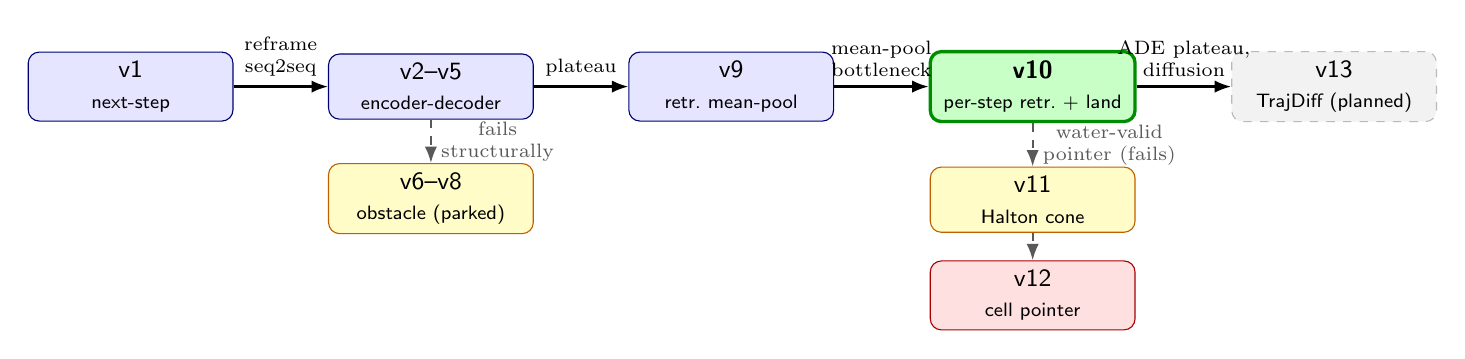
\begin{tikzpicture}[
    node distance=0.55cm and 1.2cm,
    box/.style={draw, rounded corners, minimum width=2.6cm, minimum height=0.75cm,
                align=center, font=\small\sffamily},
    prod/.style={box, fill=green!22,  draw=green!55!black, very thick},
    val/.style={box,  fill=blue!10,   draw=blue!45!black},
    plan/.style={box, fill=gray!10,   draw=gray!55, dashed},
    park/.style={box, fill=yellow!22, draw=orange!75!black},
    abandon/.style={box, fill=red!12, draw=red!65!black},
    arr/.style={-{Latex[scale=0.9]}, thick},
    weak/.style={-{Latex[scale=0.9]}, thick, dashed, gray!70!black},
  ]
  \node[val]               (v1)    {v1 \\ \scriptsize next-step};
  \node[val,  right=of v1] (v25)   {v2--v5 \\ \scriptsize encoder-decoder};
  \node[park, below=of v25] (v678) {v6--v8 \\ \scriptsize obstacle (parked)};
  \node[val,  right=of v25] (v9)   {v9 \\ \scriptsize retr.\ mean-pool};
  \node[prod, right=of v9]  (v10)  {\textbf{v10} \\ \scriptsize per-step retr.\ + land};
  \node[park, below=of v10] (v11)  {v11 \\ \scriptsize Halton cone};
  \node[abandon, below=of v11, yshift=0.2cm] (v12) {v12 \\ \scriptsize cell pointer};
  \node[plan, right=of v10] (v13)  {v13 \\ \scriptsize TrajDiff (planned)};

  \draw[arr] (v1)  -- node[midway, above, font=\scriptsize, align=center]
                       {reframe\\seq2seq} (v25);
  \draw[weak] (v25) -- node[midway, right, font=\scriptsize, align=center]
                        {fails\\structurally} (v678);
  \draw[arr] (v25) -- node[midway, above, font=\scriptsize, align=center]
                       {plateau}                                (v9);
  \draw[arr] (v9)  -- node[midway, above, font=\scriptsize, align=center]
                       {mean-pool\\bottleneck}                  (v10);
  \draw[weak] (v10) -- node[midway, right, font=\scriptsize, align=center]
                        {water-valid\\pointer (fails)}          (v11);
  \draw[weak] (v11) -- (v12);
  \draw[arr] (v10) -- node[midway, above, font=\scriptsize, align=center]
                       {ADE plateau,\\diffusion}                (v13);
\end{tikzpicture}
\caption{Design lineage of the twelve model iterations.
         Solid arrows denote successful continuations (the next version
         addresses a bottleneck identified in the previous one).
         Dashed arrows denote pivots into a parked or abandoned branch.
         Colour key: green = production, blue = validated/superseded,
         yellow = parked, red = abandoned, grey = planned.
         The main productive trajectory of the project is the horizontal
         spine v1 $\rightarrow$ v2--v5 $\rightarrow$ v9 $\rightarrow$ v10.}
\label{fig:evolution}
\end{figure}

\subsection{Notation and glossary}
\label{sec:glossary}

Project-specific terms are listed here for quick reference;
all are defined in context where first used.

\begin{description}
\item[\textbf{AIS}]
Automatic Identification System.  Mandatory ship-tracking radio signal
broadcasting position, speed, heading, and vessel category at intervals of
seconds to minutes.
\item[\textbf{MMSI}]
Maritime Mobile Service Identity. Nine-digit numeric ID assigned to each AIS
transponder; used as the train/val split key (by \emph{root MMSI}) to
prevent leakage between segments of the same physical vessel.
\item[\textbf{GSHHS}]
Global Self-consistent Hierarchical High-resolution Shoreline. Vector
shoreline dataset~\cite{wessel1996gshhs} from which the land-water boundary
of this project is derived.
\item[\textbf{\ade{}}]
Average Displacement Error. Mean Euclidean distance (in metres)
between predicted and ground-truth waypoints across all 128 time steps
of all evaluated routes. The headline metric throughout.
\item[\textbf{\fde{}}]
Final Displacement Error. Euclidean distance between the predicted and
ground-truth \emph{final} waypoint. Driven to $\approx 0$ by linear
endpoint correction in all v2+ models.
\item[\textbf{Great-circle (GC)}]
Geodesic arc baseline: 128 uniformly-spaced points on the shortest line
between start and end. Geometric lower bound on route effort.
\item[\textbf{Retrieval-top-1}]
Zero-training baseline that returns, verbatim, the single nearest
historical training route by 5-D KNN over (start, end, vessel-type).
\item[\textbf{Teacher forcing}]
Training mode where the autoregressive decoder receives ground-truth
positions as input at every step. Cheap in compute, but diverges from
inference distribution.
\item[\textbf{Scheduled sampling}]
Exposure-bias mitigation~\cite{bengio2015scheduled}: during training,
each decoder step independently uses the model's own previous prediction
with probability $p_\text{ss}$ and the ground-truth otherwise.
\item[\textbf{Exposure bias}]
The train/inference distribution mismatch caused by teacher forcing:
the model has only ever seen ground-truth context at training time but
must consume its own (noisier) predictions at inference, compounding
errors over long rollouts.
\item[\textbf{Autoregressive (AR) rollout}]
Inference procedure where the model generates one waypoint at a time,
feeding each prediction back as input for the next step --- in this
project, 128 sequential decoder calls per generated route.
\item[\textbf{Causal mask}]
Triangular attention mask in a Transformer that prevents position $t$
from attending to positions $> t$, enabling next-token prediction.
\item[\textbf{Cross-attention}]
Attention layer in an encoder-decoder Transformer where the decoder
attends to the encoder's memory tokens; used here to consume the
(start, end, vessel-type, retrieved-routes) conditioning.
\item[\textbf{Encoder-decoder Transformer}]
Architecture pairing a bidirectional Transformer encoder
(condition $\to$ memory) with a causal decoder
(memory $+$ past tokens $\to$ next token); the backbone of v2--v10.
\item[\textbf{Signed-distance field (SDF)}]
Scalar field over $\mathbb{R}^2$ whose value at point $p$ is the signed
distance to the nearest land/water boundary.
\textbf{Positive = land, negative = water} throughout this project.
\item[\textbf{Water-cell graph}]
Boolean raster at $0.005^\circ$ resolution (the fine grid)
marking which cells satisfy $\text{sdf}_\text{km} \le -0.5$,
plus 4-connectivity edges between adjacent water cells.
Domain of the WaterRouter A* search.
\item[\textbf{Linear endpoint correction}]
After AR rollout, distributes the residual endpoint error
$r = \text{pos}^T_\text{gt} - \text{pos}^T_\text{pred}$ linearly across
all 128 waypoints (frac $i/(T-1)$). Drives \fde{} to $\approx 0$
without retraining.
\item[\textbf{WaterRouter snap-only}]
Post-processor that snaps each on-land predicted waypoint to its
nearest connected fine-grid water cell via BFS (no inter-point routing).
Production water-validity layer; see Section~\ref{sec:water-router}.
\item[\textbf{DDPM / DDIM}]
Denoising Diffusion Probabilistic / Implicit Models~\cite{ho2020denoising,song2021ddim}:
the diffusion framework underlying the planned v13 (Section~\ref{sec:future}).
\item[\textbf{Classifier-free guidance (CFG)}]
Inference-time mixing of conditional and unconditional diffusion noise
predictions~\cite{ho2022classifier} that strengthens conditioning at
the cost of sample diversity. Planned for v13.
\item[\textbf{DiT}]
Diffusion Transformer~\cite{peebles2023dit} --- a Transformer block
modulated by adaLN-Zero conditioning on the diffusion timestep $t$.
The denoising backbone of v13.
\end{description}

% =====================================================================
\section{Background}
\label{sec:background}

\subsection{Transformer encoder and encoder-decoder}
\label{sec:bg-transformer}

The Transformer~\cite{vaswani2017attention} replaced recurrent networks as the
standard sequence-modelling primitive.
A \emph{Transformer encoder} is a stack of identical layers; each layer applies
multi-head self-attention followed by a position-wise feed-forward network (FFN).
Self-attention computes, for each token $i$, a weighted sum of all tokens' values:
\[
  \text{Attn}(Q,K,V) = \text{softmax}\!\left(\tfrac{QK^\top}{\sqrt{d_k}}\right)V,
\]
where $Q$, $K$, $V$ are query, key, and value projections.
A causal (triangular) mask restricts each token to attend only to past tokens,
enabling autoregressive generation.

An \emph{encoder-decoder} Transformer pairs an encoder that produces a context
\emph{memory} with a decoder that generates outputs token-by-token through
cross-attention to that memory.
This architecture underlies v2--v10 of this project.

\subsection{Autoregressive generation and exposure bias}

In autoregressive generation, the decoder produces position $t+1$ from all
previously generated positions.
During training with \emph{teacher forcing}, the decoder receives ground-truth
positions as input.
At inference, it receives its own predictions, creating a distribution mismatch
(exposure bias) that compounds errors over long rollouts.
\emph{Scheduled sampling}~\cite{bengio2015scheduled} mitigates this by
probabilistically substituting self-predictions for ground-truth inputs during
training.

\subsection{Denoising diffusion models}
\label{sec:bg-diffusion}

Denoising Diffusion Probabilistic Models (DDPM)~\cite{ho2020denoising} define a
\emph{forward process} that gradually adds Gaussian noise to a data sample $x_0$:
\[
  x_t = \sqrt{\bar\alpha_t}\, x_0 + \sqrt{1-\bar\alpha_t}\,\varepsilon,
  \qquad \varepsilon \sim \mathcal{N}(0,I),
\]
where $\bar\alpha_t$ follows a cosine schedule over $T=1000$ steps.
A neural network learns to predict $\varepsilon$ (the ``noise'') given $x_t$ and $t$.
Denoising Diffusion Implicit Models (DDIM)~\cite{song2021ddim} accelerate sampling
to 20--50 steps by reusing predicted-noise estimates across timesteps.
Classifier-free guidance (CFG)~\cite{ho2022classifier} mixes conditional and
unconditional noise predictions at inference:
\[
  \hat\varepsilon = \varepsilon_\text{uncond} + w\,(\varepsilon_\text{cond} -
                   \varepsilon_\text{uncond}), \quad w > 1,
\]
steering the sample toward a conditioning signal.
Diffusion Transformers (DiT)~\cite{peebles2023dit} replace U-Net backbones with
Transformer blocks modulated by adaptive layer normalisation (adaLN-Zero).

\subsection{Signed-distance fields}

A signed-distance field (SDF) assigns to each point $p \in \mathbb{R}^2$ a scalar
$\text{sdf}(p)$ whose absolute value is the shortest distance to a reference
boundary $\partial S$, and whose sign indicates which side of the boundary $p$ is on.
In this project, \textbf{positive} values indicate land (inside the GSHHS polygon $S$)
and \textbf{negative} values indicate water.
The SDF is precomputed once from the GSHHS shoreline~\cite{wessel1996gshhs} at
$0.05^\circ$ resolution (Section~\ref{sec:land-sdf}).

% =====================================================================
\section{Dataset and Experimental Setup}
\label{sec:setup}

\subsection{Data source and filtering}

The dataset is twelve months of US-region NOAA AIS broadcasts from 2024,
covering vessel types 60--89 (passenger, cargo, tanker, and similar commercial
classes) within the bounding box
$\text{lon} \in [-125^\circ, -60^\circ]$,
$\text{lat} \in [10^\circ, 55^\circ]$.
Raw pings are filtered by \texttt{prepare\_data.py}: minimum track length 50 pings,
maximum inter-ping jump 2\,km, maximum gap 60\,min,
turn-segmentation at headings exceeding $150^\circ$, minimum average speed
1\,km/h, minimum total distance 5\,km.
Approximately 97\,\% of raw pings are removed (80\,\% by vessel-type filter alone).

For the conditional route-generation models (v2 onward), tracks are resampled
to exactly 128 points by uniform arc-length interpolation using
\texttt{prepare\_trajgen.py}, producing a dataset of 207{,}000 routes stored as
\texttt{trajgen\_128.npz}; each entry is a $(128 \times 2)$ array of normalised
(lon, lat) values paired with metadata (start, end, vessel type).
A cleaned subset \texttt{trajgen\_128\_clean.npz} is described in
Section~\ref{sec:e1}.
The \textbf{next-step prediction models (v1, Section~\ref{sec:v1}) operate
directly on the raw irregularly-sampled tracks and do not resample}; their
training corpus is the post-filter CSV \texttt{AIS\_2024\_gt80.csv}
(tracks of $>$80 pings).

\begin{figure}[ht]
\centering
\begin{subfigure}[t]{0.96\linewidth}
  \centering
  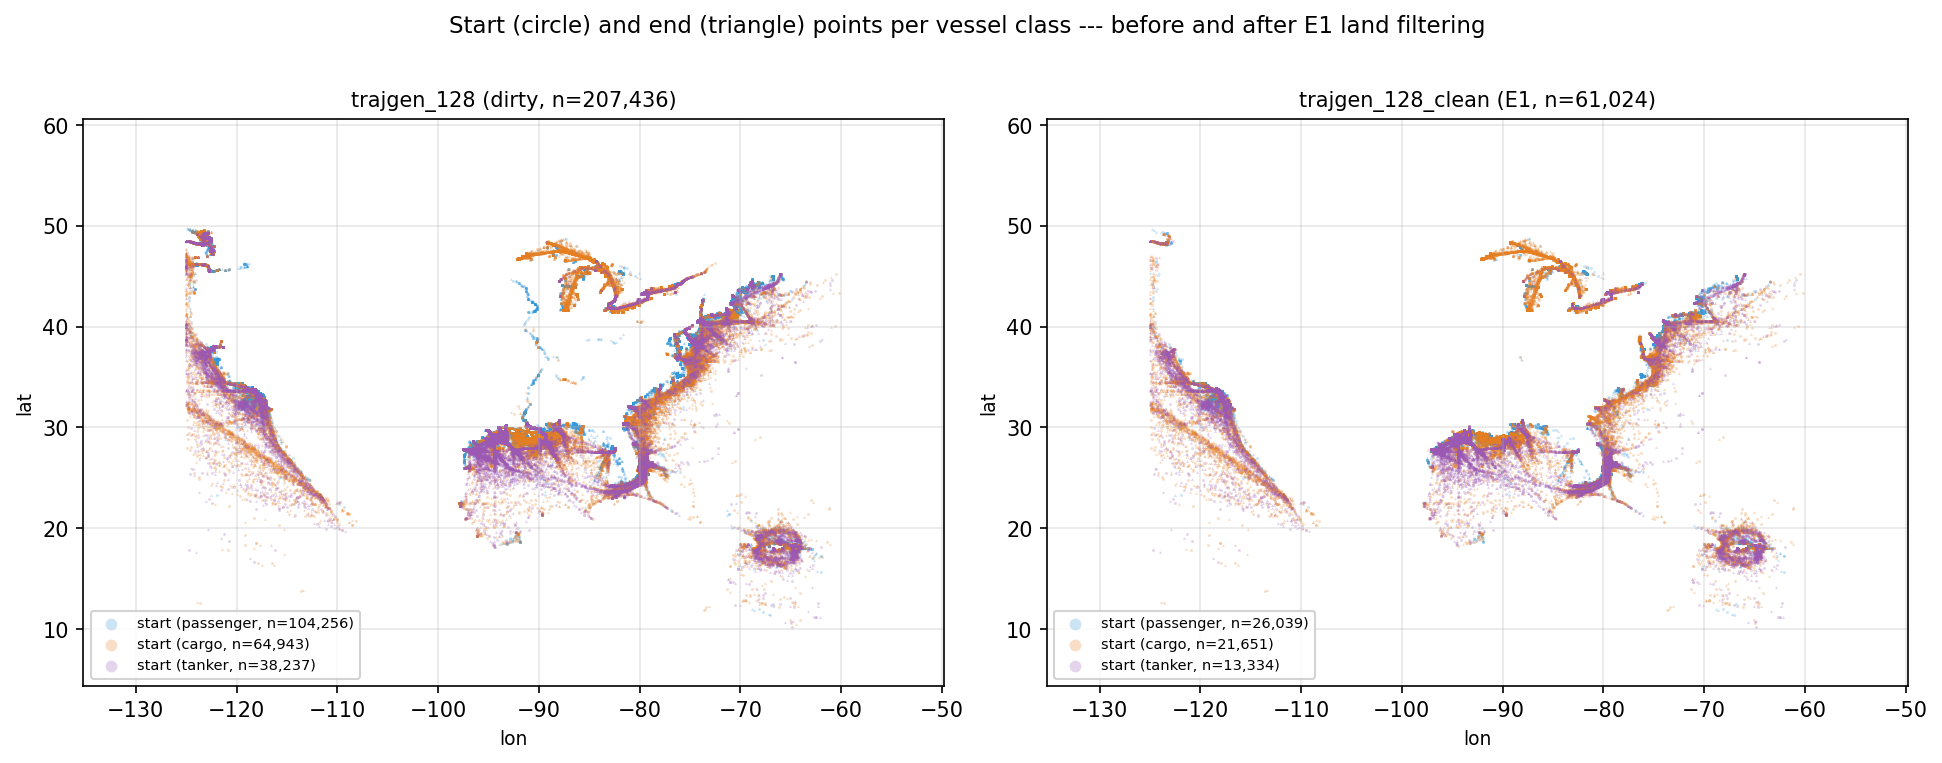
\includegraphics[width=\linewidth]{figures/data_start_end.png}
  \caption{Start (circle) and end (triangle) points of every track,
           coloured by vessel class, shown side-by-side for the dirty
           dataset (left, $n=207\,436$) and the E1-cleaned subset (right,
           $n=61\,024$).  Cleaning removes inland-rivers and tight-coastal
           tracks without changing the overall coverage shape.}
  \label{fig:data-start-end}
\end{subfigure}\\[0.3em]
\begin{subfigure}[t]{0.59\linewidth}
  \centering
  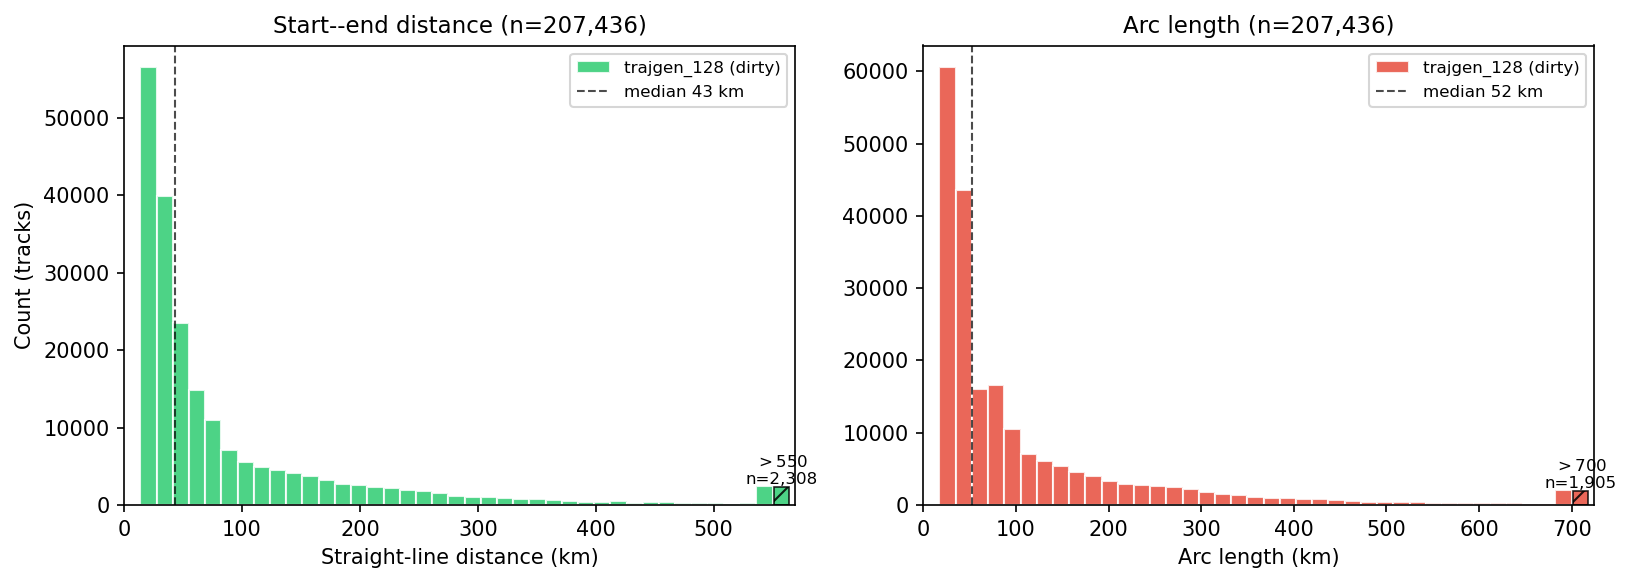
\includegraphics[width=\linewidth]{figures/data_distributions.png}
  \caption{Distributions of straight-line distance and arc length.
           X-axis clipped at the 99th percentile; the hatched bar on the
           right of each panel aggregates all tracks beyond the clip.}
  \label{fig:data-dist}
\end{subfigure}\hfill
\begin{subfigure}[t]{0.38\linewidth}
  \centering
  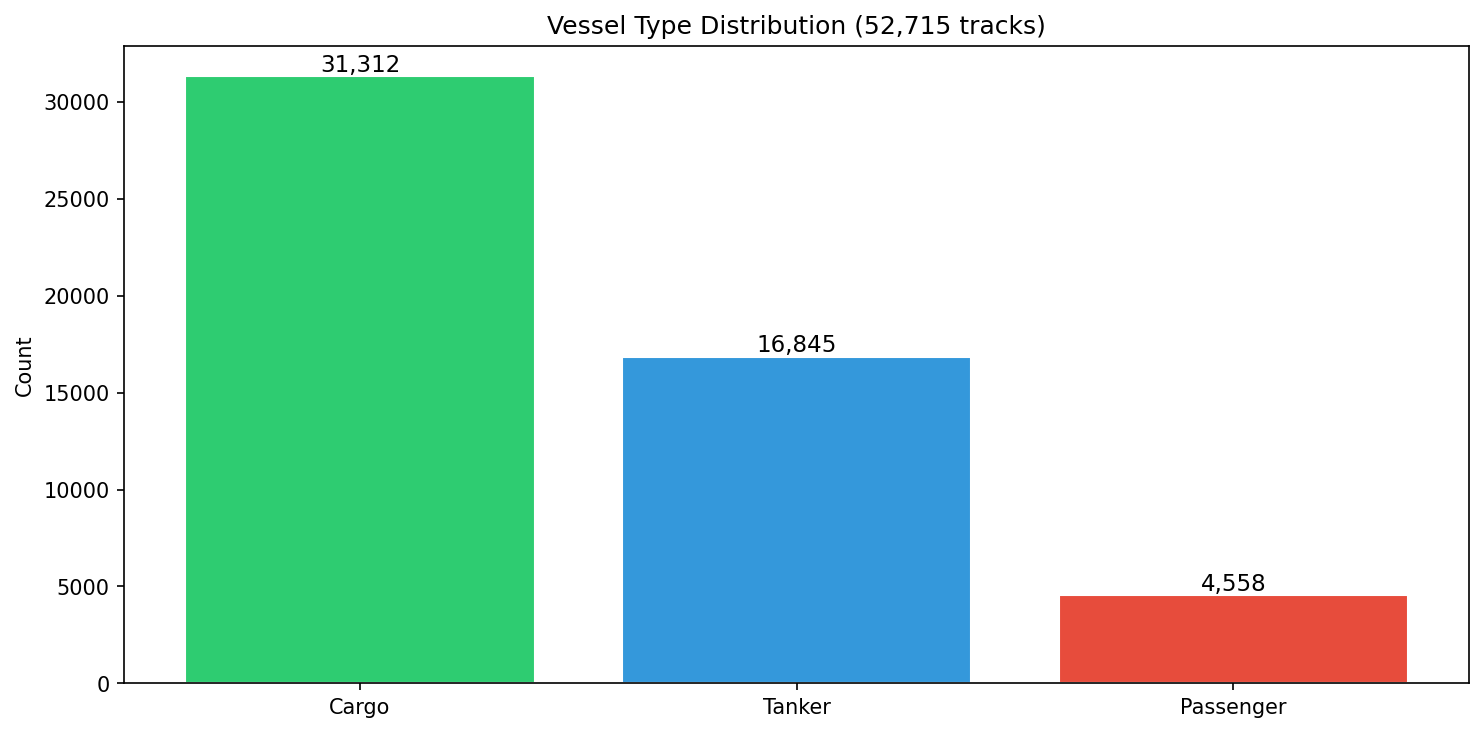
\includegraphics[width=\linewidth]{figures/data_vessel_types.png}
  \caption{Vessel-type mix in the 128-point dataset.}
  \label{fig:data-vtypes}
\end{subfigure}
\caption{Dataset overview of \texttt{trajgen\_128.npz}.
         207k tracks spread across the US Atlantic, Gulf, and Pacific
         coasts; 45\,\% passenger, 24\,\% cargo, 14\,\% tanker;
         median straight-line distance 43\,km with a long tail to
         2000\,km (Section~\ref{sec:contributions} bucketed evaluation
         uses cutoffs 50\,km and 500\,km to separate these regimes).}
\label{fig:data-overview}
\end{figure}

\subsection{Evaluation protocol}

All trajectory-generation experiments are evaluated on a fixed set of
$n=500$ validation routes sampled with \texttt{seed=42}; results for the
production system are additionally aggregated over the seed set
$\{0,1,2,42,123\}$ in Section~\ref{sec:ranking} and
Appendix~\ref{app:variance} to confirm the headline figure is not
seed-cherry-picked.
The train/validation split is by \emph{root MMSI}: all AIS segments of the
same physical vessel (identified by stripping batch prefix and segment suffix
from the synthetic vessel ID) land entirely in train or entirely in validation,
preventing data leakage.

\paragraph{Threats to validity.} Three caveats apply to all comparisons below
and the reader should keep them in mind when interpreting differences between
model versions:
\begin{itemize}
  \item \textbf{No held-out test set.} The pipeline uses a single train/val
        split (\texttt{val\_frac=0.15}); the validation set is used both for
        epoch selection (\texttt{best.pt} is the checkpoint with lowest
        validation loss) and for the headline figures in the tables that
        follow. Reported numbers are therefore validation-set performance,
        not test-set performance, and may be mildly optimistic on the
        per-model level (model selection bias). A clean held-out test split
        was not introduced because the project's failure-driven design loop
        relied on iterating against validation-rollout \ade{}; this is a
        deliberate cost flagged in Section~\ref{sec:open-challenges}.
  \item \textbf{One training seed per model.} Each model version (v1, v5,
        v9, v10, v11, v12, etc.) was trained exactly once. The five-seed
        variance reported in Appendix~\ref{app:variance} sweeps only the
        \emph{evaluation subsample seed} on the already-trained v10
        checkpoint. Differences between models within $\sim$225\,m
        (the v10 subsample-noise $\sigma$) may not be reproducible across
        independent training runs.
  \item \textbf{Mixed evaluation-seed counts across rows.}
        For every comparison table that pits v10 against earlier models
        (v5, v9, retrieval-top-1, great-circle), the v10 row is reported at
        \texttt{seed=42} so that the model-vs-model comparison is on the same
        500-route subsample; the five-seed mean from
        Appendix~\ref{app:variance} is reserved for the abstract and the
        production use-case ranking caption (Section~\ref{sec:ranking}).
        Comparisons across the canonical seed are therefore paired (same 500
        routes, same harness), but no $p$-value or paired statistical test
        is computed.
\end{itemize}

Two primary metrics are reported throughout:
\begin{itemize}
  \item \textbf{\ade{} (Average Displacement Error)}: mean Euclidean distance
    in metres between predicted and ground-truth waypoints, averaged over all
    128 steps and all 500 validation routes.
  \item \textbf{\fde{} (Final Displacement Error)}: Euclidean distance in metres
    between predicted and ground-truth \emph{final} waypoints.
    Linear endpoint correction (Section~\ref{sec:endpoint-correction}) drives
    \fde{} to near zero for all AR models.
\end{itemize}

Length-bucketed \ade{} further breaks down results into short ($<$50\,km),
medium (50--500\,km), and long ($>$500\,km) route categories.

Land-crossing metrics are:
$\text{land\%@}d$ (fraction of predicted waypoints with $\text{sdf} > d$~km)
and $\text{cross\%@}d$ (fraction of trajectories with at least one waypoint
exceeding the threshold).

\subsection{Hardware and software}

Training runs were executed on heterogeneous hardware (CUDA GPU, Apple Silicon MPS,
and CPU), handled by device auto-detection logic consistent across all model versions.
All models are implemented in PyTorch.
Inference latency for v10 + WaterRouter snap-only is approximately
50\,ms per query on a single CPU core.

\subsection{Baselines}

\textbf{Great-circle (GC)}: 128 uniformly-spaced points along the geodesic arc
between start and end.
\ade{} = 8226\,m on \texttt{trajgen\_128.npz}; serves as the lower-effort
geometric baseline throughout.

\textbf{Retrieval-top-1}: returns the single most similar training route verbatim,
selected by 5-D KNN over (start, end, vessel-type).
\ade{} = 6470\,m on \texttt{trajgen\_128.npz} (seed=42 evaluation harness);
a zero-training baseline showing the information value of historical traffic.

% =====================================================================
\section{Technical Contributions}
\label{sec:contributions}

\subsection{v1 -- Next-step displacement prediction}
\label{sec:v1}

\subsubsection{Architecture}

The first model treated trajectory modelling as a next-step regression problem:
given the past $L=120$ ping triples $(lon, lat, \Delta t)$, predict the
displacement $(\Delta lon, \Delta lat)$ to the next ping.
The implementation is a Transformer encoder with a causal (triangular) mask
(\texttt{src/model.py}, class \texttt{AISTransformer}).
Each timestep is encoded as a 5-dimensional vector:
\[
  x_i = [lon_i^\text{norm},\ lat_i^\text{norm},\ \log(\Delta t_i)^\text{norm},
          \ \Delta lon_i^\text{norm},\ \Delta lat_i^\text{norm}]
\]
plus a learned 8-dimensional vessel-type embedding added at every step.
Displacement is chosen as the regression target rather than absolute position
because it has small, zero-centred variance independent of geographic location,
keeping the per-coordinate target distribution stable across the dataset.
Three independent scalers (position, log-$\Delta t$, displacement) are fitted on
the training partition only.

\textbf{Bidirectional attention is unsafe for next-step prediction.}
An early bidirectional variant (mean pooling of encoder outputs) attained
much lower training MSE than the causal variant; closer inspection revealed
the model was attending to \emph{future} positions and degenerating into a
copy operator, producing apparently-perfect training curves but useless
rollouts.  All subsequent v1 runs use causal masking, and the v2+ ladder uses
teacher-forced training with autoregressive inference for the same reason
(exposure bias is preferable to information leakage).

\begin{figure}[ht]
\centering
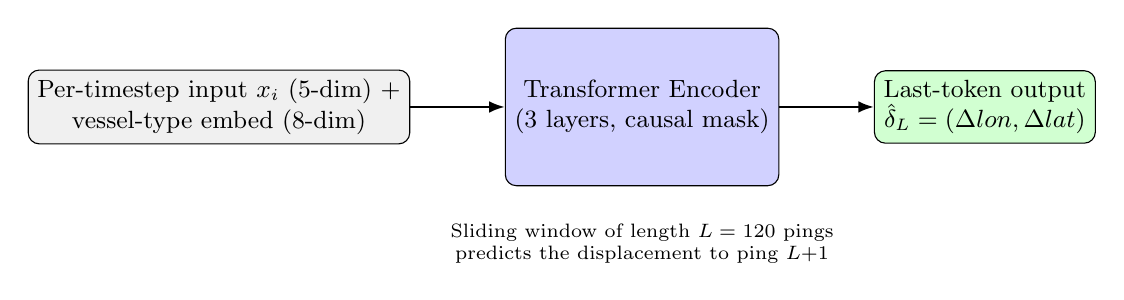
\begin{tikzpicture}[
    node distance=0.55cm and 1.0cm,
    box/.style={draw, rounded corners, minimum width=2.4cm, minimum height=0.55cm,
                align=center, font=\small},
    arr/.style={-{Latex[scale=0.85]}, thick},
  ]
  % Input feature stack (per timestep)
  \node[box, fill=gray!12, minimum width=4.2cm] (inp)
        {Per-timestep input $x_i$ (5-dim) +\\
         vessel-type embed (8-dim)};
  % Encoder
  \node[box, fill=blue!18, right=1.2cm of inp, minimum width=3.2cm,
        minimum height=2.0cm] (enc)
        {Transformer Encoder\\(3 layers, causal mask)};
  % Last-token output
  \node[box, fill=green!18, right=1.2cm of enc, minimum width=2.4cm]
        (out) {Last-token output\\$\hat\delta_L = (\Delta lon,\Delta lat)$};
  % Note below
  \node[align=center, font=\scriptsize, below=0.35cm of enc]
        {Sliding window of length $L=120$ pings\\
         predicts the displacement to ping $L{+}1$};

  \draw[arr] (inp.east) -- (enc.west);
  \draw[arr] (enc.east) -- (out.west);
\end{tikzpicture}
\caption{v1 next-step regression architecture.
         A causal Transformer encoder reads a 120-ping window and emits one
         displacement prediction from the last position's hidden state.
         The per-timestep input concatenates absolute position, $\log\Delta t$,
         the previous displacement, and a learned vessel-type embedding.}
\label{fig:v1-arch}
\end{figure}

\subsubsection{Iteration path}

The v1 line is best understood as a sequence of targeted ablations, each
motivated by a specific hypothesis about why per-step accuracy was not
improving:

\textit{Stage 1 --- causal vs.\ bidirectional.}
Initial training with bidirectional attention produced suspiciously low
training MSE.  The bidirectional model was reading future positions and
copying them; switching to a causal mask immediately raised training MSE
to a believable range while restoring meaningful rollout behaviour.

\textit{Stage 2 --- displacement vs.\ velocity.}
A first round of training used absolute position as the regression target.
Variance was dominated by geographic location (Atlantic vs.\ Gulf) rather
than by the actual prediction task, and gradients were correspondingly
noisy.  Switching to a \emph{displacement} target $(\Delta lon, \Delta lat)$
centred the distribution at zero and stabilised optimisation.  A further
variant using \emph{velocity} (displacement divided by $\Delta t$, so the
target is ping-interval invariant) was trained in \texttt{train\_vel.py};
it converged comparably but did not change the overall conclusion.

\textit{Stage 3 --- vessel-type conditioning.}
A learned 8-dimensional embedding over the 28 AIS vessel codes is added at
every timestep.  Without it, the model defaults to passenger-vessel
dynamics; with it, ablations confirmed cargo / tanker tracks were predicted
with the expected lower turn rates.

\textit{Stage 4 --- auxiliary features.}
Two auxiliary feature streams were prototyped: \emph{lighthouse-distance}
features (distances to the three nearest lighthouses, as a proxy for
``how coastal is this ping''), and \emph{nearest-vessel} features (distance
and bearing to the nearest concurrent vessel, as a proxy for collision
context).  Both regressed performance: see Table~\ref{tab:v1}, last row
(lighthouse).  The features were redundant with absolute position --- the
encoder could already infer ``coastal'' from $(lon, lat)$ --- and added
noise without adding signal.

\textit{Stage 5 --- multi-step rollout evaluation.}
A separate evaluation harness (\texttt{eval\_multistep.py}) was added to
predict horizons $H = 1, 2, 5, 10, 20$ autoregressively, accumulating
errors.  At every horizon, the model diverged \emph{faster} than the
constant-velocity baseline --- a clear signature of exposure bias on a near-linear
target.  This was the result that prompted the move from per-step
regression to full-sequence generation in v2.

\subsubsection{Result}

\begin{table}[ht]
\centering
\caption{v1 next-step model vs.\ constant-velocity (CV) baseline.
         ADE in metres; lower is better.}
\label{tab:v1}
\begin{tabular}{lrr}
\toprule
Run & CV \ade{} & Model \ade{} \\
\midrule
12-month full dataset    & 50.7 & 50.8 \\
Open-sea filtered        & 47.0 & 47.5 \\
Open-sea + lighthouse    & 47.0 & 48.6 \\
\bottomrule
\end{tabular}
\end{table}

After all five iteration stages, the model matches but never beats the
constant-velocity baseline (Table~\ref{tab:v1}).  Multi-step rollout
diverged faster than CV at horizons 5, 10, and 20.  Lighthouse features
made results strictly worse; nearest-vessel features did not change them.

\subsubsection{Lesson}

Open-sea AIS tracks are nearly linear at 3-minute pings: the CV predictor is
near-optimal on post-turn-segmented data.
More broadly, \textbf{per-step accuracy in normalised MSE is not predictive of
trajectory-level error}.
This finding recurs repeatedly through v2--v12 and is the single most important
cross-cutting lesson of the project.

\noindent\textit{Training-duration note.}
Among the eight v1 runs, four reached their planned epoch count
(\texttt{12mo\_seq120}, \texttt{12mo\_seq120\_opensea},
\texttt{12mo\_seq120\_opensea\_lh}, \texttt{4wk\_seq80\_e40}),
and four were stopped early once the CV-tie conclusion was unambiguous:
\texttt{12mo\_seq120\_bs384} (6/40, batch-size experiment),
\texttt{12mo\_seq120\_lh} (15/40, lighthouse features regressed),
\texttt{4wk\_seq120\_e30} (31/40, compute budget),
and \texttt{12mo\_seq80} (never run; queued config left for completeness).
The headline number for v1 is the fully-trained
\texttt{12mo\_seq120\_opensea} (40/40 epochs).

\subsection{v2--v5 -- Encoder-decoder trajectory generator}
\label{sec:v2v5}

\subsubsection{Reframing as seq2seq}

The pivot from v1 to v2 reframed the task as a \emph{sequence-to-sequence}
generation problem: given (start, end, vessel\_type), generate a full 128-point
route.
The dataset was rebuilt by \texttt{prepare\_trajgen.py}, which resamples each
track to exactly 128 arc-length-uniform waypoints and discards time-delta
information (vessel speed is recovered implicitly through the vessel-type embedding).

\subsubsection{Architecture (\texttt{src/model\_gen.py})}

\begin{figure}[ht]
\centering
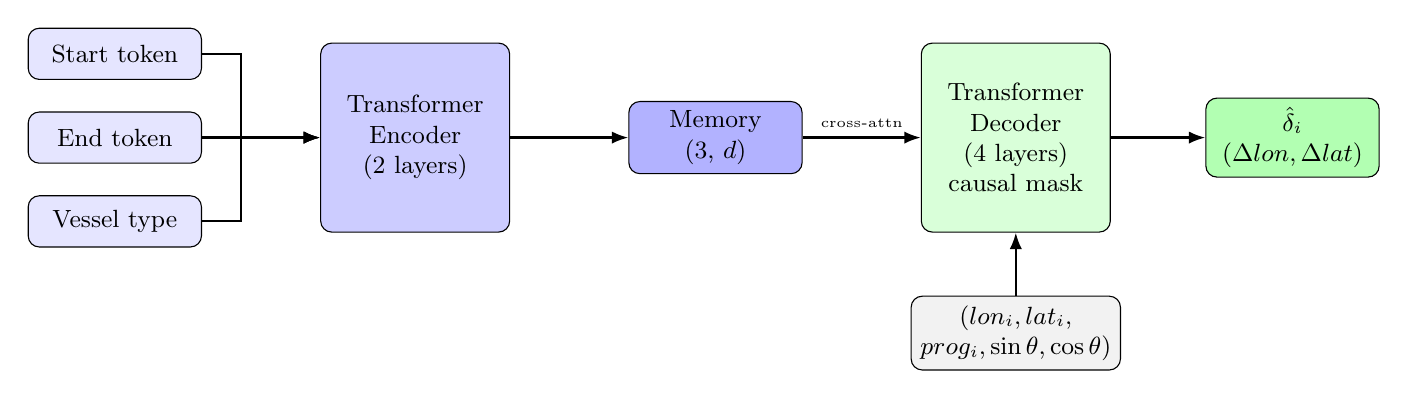
\begin{tikzpicture}[
    node distance=0.8cm and 1.5cm,
    box/.style={draw, rounded corners, minimum width=2.2cm, minimum height=0.65cm,
                align=center, font=\small},
    arr/.style={-{Latex[scale=0.9]}, thick},
  ]
  % Encoder tokens
  \node[box, fill=blue!10]  (start) {Start token};
  \node[box, fill=blue!10, below=0.4cm of start] (end) {End token};
  \node[box, fill=blue!10, below=0.4cm of end]   (vtype) {Vessel type};
  % Encoder
  \node[box, fill=blue!20, right=1.5cm of end, minimum width=2.4cm,
        minimum height=2.4cm, align=center] (enc) {Transformer\\Encoder\\(2 layers)};
  % Memory
  \node[box, fill=blue!30, right=1.5cm of enc] (mem) {Memory\\(3, $d$)};
  % Decoder
  \node[box, fill=green!15, right=1.5cm of mem, minimum height=2.4cm,
        minimum width=2.4cm] (dec) {Transformer\\Decoder\\(4 layers)\\causal mask};
  % Output
  \node[box, fill=green!30, right=1.2cm of dec] (out) {$\hat\delta_i$\\$(\Delta lon,\Delta lat)$};
  % Input to decoder
  \node[box, fill=gray!10, below=0.8cm of dec] (inp) {$(lon_i, lat_i,$\\$prog_i, \sin\theta,\cos\theta)$};

  \draw[arr] (start.east) -- ++(0.5,0) |- (enc.west);
  \draw[arr] (end.east)   -- (enc.west);
  \draw[arr] (vtype.east) -- ++(0.5,0) |- (enc.west);
  \draw[arr] (enc.east)   -- (mem.west);
  \draw[arr] (mem.east)   -- (dec.west) node[midway,above,font=\tiny]{cross-attn};
  \draw[arr] (inp.north)  -- (dec.south);
  \draw[arr] (dec.east)   -- (out.west);
\end{tikzpicture}
\caption{v4/v5 encoder-decoder architecture. The encoder produces 3 context tokens
         from start, end, and vessel-type conditioning.  The decoder generates the
         128-point route autoregressively via causal self-attention and cross-attention
         to the encoder memory. Input features include bearing-to-destination
         $(\sin\theta, \cos\theta)$ added in v4.}
\label{fig:v4-arch}
\end{figure}

\textbf{Encoder.}  Three conditioning tokens (start, end, vessel-type), each
projected through a linear layer to $d_\text{model}$, plus learned token-type
embeddings to distinguish their roles.
Output: memory $\in \mathbb{R}^{3 \times B \times d_\text{model}}$.

\textbf{Decoder.}  Consumes a per-step input and generates 128 waypoints
autoregressively.
Each step's input (3-dim for MVP/v2/v3; 5-dim for v4/v5 with bearing) is projected
to $d_\text{model}$, summed with sinusoidal positional encoding, and passed through
four Transformer decoder layers (causal self-attention + cross-attention to encoder memory).
A linear head emits predicted displacement $(\Delta lon, \Delta lat)$;
the next position is recovered as:
\[
  \text{pos}_{i+1} = \text{pos}_i + \delta_\text{scaler}^{-1}(\hat\delta_i).
\]

\textbf{Loss.}
\begin{equation}
  \mathcal{L} = \mathcal{L}_\delta + \lambda_\text{end}\,\mathcal{L}_\text{endpoint}
              + \lambda_\text{smooth}\,\mathcal{L}_\text{smooth},
  \label{eq:gen-loss}
\end{equation}
where $\mathcal{L}_\delta$ is Huber loss on predicted vs.\ ground-truth deltas,
$\mathcal{L}_\text{endpoint} = \|\text{pos}^T_\text{pred} - \text{pos}^T_\text{gt}\|^2$,
and $\mathcal{L}_\text{smooth} = \frac{1}{T-2}\sum_i\|\text{accel}_i\|^2$ penalises
second-order acceleration.
MVP configuration: $\lambda_\text{end}=10$, $\lambda_\text{smooth}=1.0$.

\subsubsection{Linear endpoint correction}
\label{sec:endpoint-correction}

After autoregressive rollout, the residual endpoint error
$r = \text{pos}^T_\text{gt} - \text{pos}^T_\text{pred}$ is distributed linearly
across all 128 waypoints:
\[
  \text{pos}_i^\text{corrected} = \text{pos}_i^\text{raw} + r \cdot \frac{i}{T-1},
  \quad i = 1,\ldots,128.
\]
This drives \fde{} to near zero without retraining and is retained in every
subsequent model.

\begin{algorithm}[ht]
\caption{Linear Endpoint Correction}
\label{alg:endpoint}
\begin{algorithmic}[1]
\REQUIRE raw trajectory $\mathbf{x}^{\text{raw}}$, ground-truth endpoint $\text{pos}^T_\text{gt}$
\STATE $r \gets \text{pos}^T_\text{gt} - x^{\text{raw}}_{128}$
\FOR{$i = 1$ \textbf{to} $128$}
    \STATE $x_i^{\text{corrected}} \gets x_i^{\text{raw}} + r \cdot (i-1)/(128-1)$
\ENDFOR
\STATE \RETURN $\mathbf{x}^{\text{corrected}}$
\end{algorithmic}
\end{algorithm}

\subsubsection{Scheduled sampling (v3, v5)}

To mitigate exposure bias, v3 and v5 use \emph{scheduled sampling}~\cite{bengio2015scheduled}.
The naive step-by-step replacement was infeasible at $T=128$, so the
implementation uses a \emph{two-pass parallel} scheme:
Pass 1 runs the standard parallel teacher-forced decoder under
\texttt{torch.no\_grad()} to obtain one-step-ahead predictions;
a mixed input trajectory is constructed by selecting ground-truth or self-prediction
per step with probability $p_\text{ss}$;
Pass 2 re-runs the decoder with gradients on the mixed input.
Cost: $\approx 2\times$ standard teacher forcing vs.\ $\sim128\times$ for the naive loop.

\subsubsection{Architectural ladder results}

\begin{table}[ht]
\centering
\caption{v2--v5 architectural ladder.
         val\_delta is per-step loss in normalised delta space; ADE is evaluated by
         autoregressive rollout over 500 validation routes (seed=42).
         The architectural ladder produced no real-world ADE improvement.}
\label{tab:v2v5}
\begin{tabular}{llcccr}
\toprule
Config & Changes vs.\ MVP & $d_\text{model}$ & Enc.\ layers & val\_delta & \ade{} (m) \\
\midrule
MVP    & Baseline          & 128 & 0 & 0.086 & 6807 \\
v2     & $\lambda_\text{end}=50$   & 128 & 0 & 0.105 & ---\textsuperscript{$\dagger$} \\
v3     & v2 + SS           & 128 & 0 & 0.105 & ---\textsuperscript{$\dagger$} \\
v4     & $d\!=\!256$, bearing feat., 2 enc.\ layers & 256 & 2 & 0.072 & 6801 \\
v5     & v4 + SS           & 256 & 2 & 0.074 & 6753 \\
\bottomrule
\end{tabular}
\vspace{0.3em}
\small\textsuperscript{$\dagger$}\,v2 and v3 used the earlier 3-dim decoder
input (no bearing feature); the live \texttt{TrajectoryGenerator} class no
longer accepts those checkpoints.  Per-step val\_delta is reported instead;
the rollout-ADE conclusion is unchanged by v4's measurement (6801\,m,
statistically indistinguishable from MVP at 6807\,m).
\end{table}

Figure~\ref{fig:ade-by-model} and Table~\ref{tab:v2v5} document the central negative finding:
a 14\,\% improvement in val\_delta (0.086 $\to$ 0.074) corresponds to a $\sim$1\,\%
improvement in \ade{} (6807 $\to$ 6753~m) that vanishes inside evaluation noise.
The entire architectural ladder produced no measurable real-world improvement.

\begin{figure}[ht]
\centering
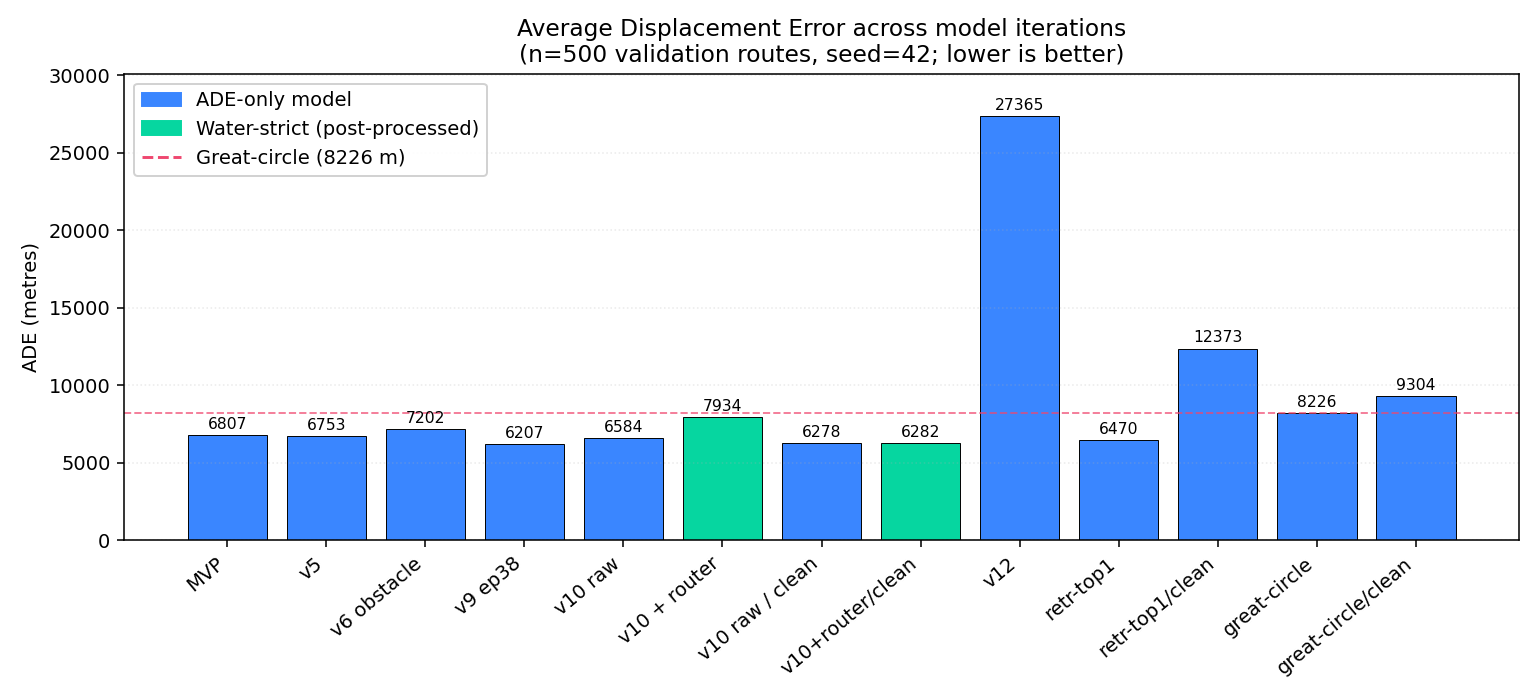
\includegraphics[width=\linewidth]{figures/ade_by_model.png}
\caption{ADE across model iterations.
         Blue bars: ADE-only models on \texttt{trajgen\_128.npz} (dirty data).
         Green bars: water-strict variants.
         Dashed red line: great-circle baseline.
         Note the logarithmic scale on the right portion of the x-axis for v12.}
\label{fig:ade-by-model}
\end{figure}

Figure~\ref{fig:motiv-v5} shows the qualitative failure mode that the
architectural ladder did not address: v5 routes whose \emph{final waypoint}
terminates inland, several tens of kilometres from any coastline.
These cases are typical of medium-length val routes where the geometry of
nearby historical traffic is the missing signal --- and are what motivated
the move to retrieval-augmented generation in v9.

\begin{figure}[ht]
\centering
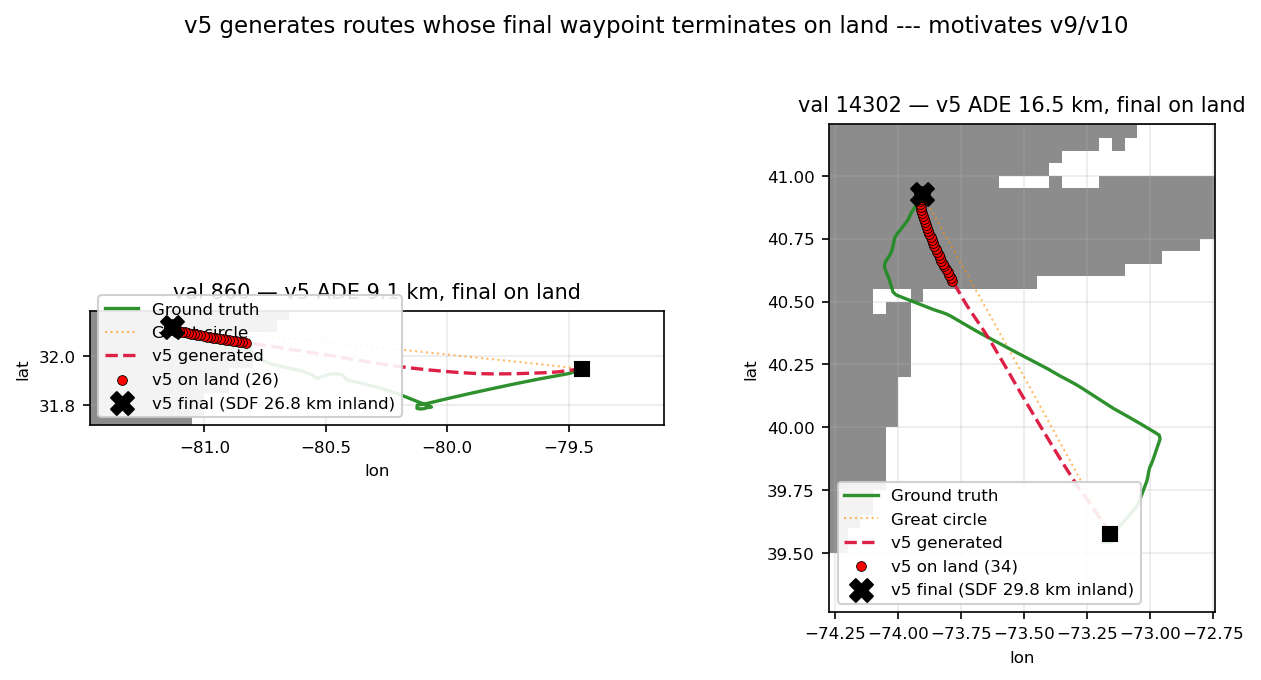
\includegraphics[width=0.95\linewidth]{figures/motiv_v5_lands_on_coast.png}
\caption{Two v5 (epoch~54) predictions whose final waypoint terminates
         on land (signed-distance to coast $>$ 25\,km inland in both cases).
         Grey blocks are land masses (rasterised GSHHS coastline at
         $0.05^\circ$); white is water.  Green solid is the ground-truth
         route, red dashed is the v5 prediction, dotted orange is the
         great-circle baseline, and the black \texttt{X} marks the v5
         final waypoint.  Red dots flag every v5 waypoint with
         $\text{sdf\_km}>0$ (on land).
         The model has no explicit notion of where land is; nothing in the
         per-step displacement loss penalises a final-waypoint excursion
         into the continental interior.  Land awareness is added in v10
         (Section~\ref{sec:v10}).}
\label{fig:motiv-v5}
\end{figure}

\noindent\textit{Training-duration note.}
Of the five v2--v5 runs, only \texttt{trajgen\_v4} reached its planned 60
epochs.
\texttt{trajgen\_mvp} stopped at 45/50 once the val\_delta plateau was
unmistakable; \texttt{trajgen\_v2} and \texttt{trajgen\_v3} stopped at 31/100
and 20/100 respectively because their plateau was visible even earlier;
\texttt{trajgen\_v5} stopped at 54/60 because the ladder's lesson (no real-world
\ade{} movement) was already established and further training was deemed
unlikely to alter the headline.

\subsection{v6, v7, v8 -- Obstacle-conditioned generation (parked)}
\label{sec:v6v7}

\subsubsection{Motivation and architecture}

v6/v7 extended the v4/v5 encoder with $K\le3$ obstacle tokens, each encoding
(centre\_lon, centre\_lat, radius\_deg) projected to $d_\text{model}$.
The training loss added a fourth term:
\begin{equation}
  \mathcal{L}_\text{obs} = \frac{1}{T}\sum_i
    \max\!\left(0,\; r + m - \|x_i - c\|\right)^2,
  \label{eq:obstacle-loss}
\end{equation}
a one-sided quadratic penalty firing when predicted waypoint $x_i$ penetrates
obstacle circle (centre $c$, radius $r$, margin $m$).
The intent was obstacle-avoidance: given exclusion zones, the decoder should route
around them.

\subsubsection{v6 --- the data leak}

\texttt{ObstacleTrajectoryGenDataset.\_\_getitem\_\_} seeded its RNG with
\texttt{self.seed + idx}, assigning the \emph{same} obstacle placement to every
sample at every epoch.
The model memorised (trajectory, obstacle) pairs; the ground-truth route never
crossed those obstacles; $\mathcal{L}_\text{obs} \equiv 0$ throughout training.
The training log showed \texttt{val\_obstacle}~$\approx 3\times10^{-5}$---not
``avoidance working'', but ``the penalty had nothing to penalise''.
Evaluation returned an avoidance rate of 0.0\,\%.

\subsubsection{v7 --- the structural failure}

Fixing the data leak (\texttt{deterministic=False} in the dataset) revealed a
deeper problem: the obstacle augmenter placed obstacles \emph{laterally offset} from
the ground-truth route, not on it.
The GT route therefore never approached the obstacle;
$\mathcal{L}_\text{obs} = 0$ on any decoder output close to GT.
The decoder cross-attended to the obstacle tokens but they carried no predictive
signal; spurious epoch-specific correlations drove val\_loss from 0.72 (epoch~5)
to 14.29 (epoch~17).

\textbf{Structural diagnosis.}
A constraint loss can only produce a gradient on training examples where the
constraint is potentially \emph{violated}.
Reviving obstacle-avoidance requires synthesising true detour trajectories
(e.g., bent great-circle routes, RRT-planned detours) as ground-truth targets---a
substantial dataset-engineering project not attempted in this work.

\noindent\textit{Training-duration note.}
\texttt{trajgen\_v6\_obstacle} ran 50/60 epochs before the RNG-leak was found;
\texttt{trajgen\_v7\_obstacle} ran 22/60 after the leak fix, at which point
the val-loss explosion (Section~\ref{sec:v6v7}) made the structural problem
unambiguous and further training was halted.
v8 was a planned hyperparameter sweep (\texttt{p\_obstacle}\,:\,$0.5\to1.0$,
richer augmenter, scheduled sampling) that was never run after the v7
analysis showed augmenter-side fixes could not address the
zero-gradient root cause.

\subsection{v9 -- Retrieval-augmented generation}
\label{sec:v9}

\subsubsection{Retrieval-top-1 gate}

Before training v9, a zero-parameter experiment was run:
for each validation query, return the nearest training route verbatim (retrieval-top-1),
where nearness is defined by 5-D KNN over
(start\_lon, start\_lat, end\_lon, end\_lat, vessel\_type).
Result: \ade{} = 5489\,m\footnote{This measurement was made on a slightly
different evaluation slice from the full seed=42 harness; the corresponding
seed=42 figure is 6470\,m.  Both are included in \texttt{results/summary.csv}.},
a 19\,\% improvement over the best trained model (v5 at 6753\,m).
This zero-training baseline validated the retrieval substrate before any parameters
were learned.

\subsubsection{Architecture (\texttt{src/model\_gen\_retrieval.py})}

v9 extends the v4 encoder with $K=5$ retrieved historical routes.
A \texttt{MeanPoolRouteEncoder} compresses each retrieved $(128\times2)$ route to a
single $d_\text{model}$-dimensional vector by mean-pooling the 128 position vectors
and projecting.
Encoder memory grows from 3 base tokens to $3 + 5 = 8$ tokens.
The decoder cross-attends to all 8.

\begin{figure}[ht]
\centering
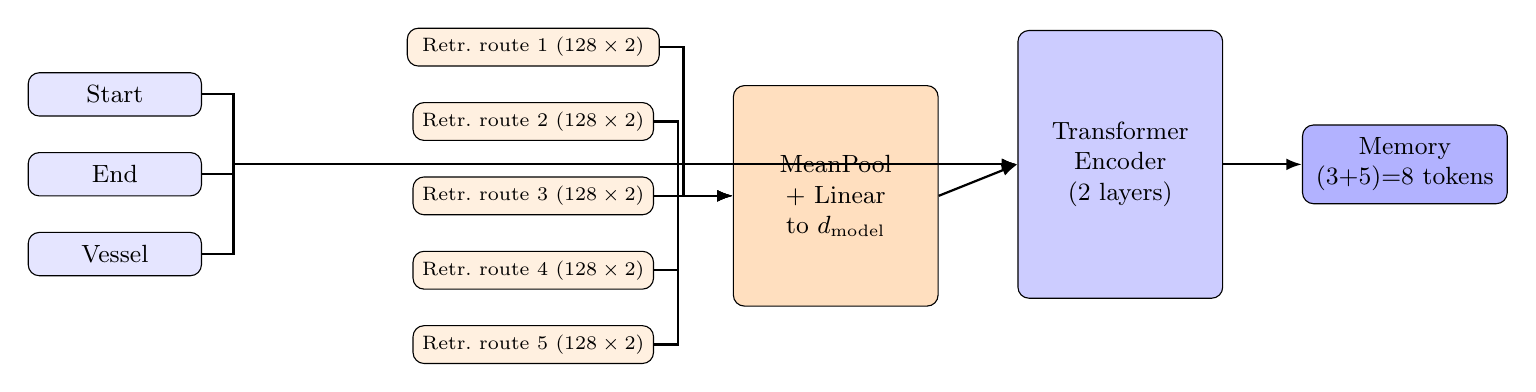
\begin{tikzpicture}[
    node distance=0.45cm and 1.0cm,
    box/.style={draw, rounded corners, minimum width=2.2cm, minimum height=0.55cm,
                align=center, font=\small},
    smallbox/.style={draw, rounded corners, minimum width=2.3cm, minimum height=0.45cm,
                     align=center, font=\scriptsize},
    arr/.style={-{Latex[scale=0.85]}, thick},
  ]
  % Base tokens
  \node[box, fill=blue!10]                       (start) {Start};
  \node[box, fill=blue!10, below=of start]       (end)   {End};
  \node[box, fill=blue!10, below=of end]         (vtype) {Vessel};
  % Retrieved routes (5 of them) on the left, with mean-pool
  \node[smallbox, fill=orange!12, right=2.6cm of start, yshift=0.6cm,
        minimum width=3.2cm] (r1) {Retr.\ route 1 $(128\times 2)$};
  \node[smallbox, fill=orange!12, below=of r1] (r2) {Retr.\ route 2 $(128\times 2)$};
  \node[smallbox, fill=orange!12, below=of r2] (r3) {Retr.\ route 3 $(128\times 2)$};
  \node[smallbox, fill=orange!12, below=of r3] (r4) {Retr.\ route 4 $(128\times 2)$};
  \node[smallbox, fill=orange!12, below=of r4] (r5) {Retr.\ route 5 $(128\times 2)$};
  % Mean-pool block
  \node[box, fill=orange!25, right=1.0cm of r3, minimum height=2.8cm, minimum width=2.6cm,
        align=center] (mp) {MeanPool\\$+$ Linear\\to $d_{\text{model}}$};
  % Encoder
  \node[box, fill=blue!20, right=1.0cm of mp, minimum width=2.6cm, minimum height=3.4cm,
        align=center, yshift=0.4cm] (enc) {Transformer\\Encoder\\(2 layers)};
  % Memory (8 tokens)
  \node[box, fill=blue!30, right=1.0cm of enc, minimum height=1.0cm,
        minimum width=2.6cm] (mem) {Memory\\$(3{+}5){=}8$ tokens};

  \draw[arr] (start.east) -- ++(0.4,0) |- (enc.west);
  \draw[arr] (end.east)   -- ++(0.4,0) |- (enc.west);
  \draw[arr] (vtype.east) -- ++(0.4,0) |- (enc.west);
  \draw[arr] (r1.east) -- ++(0.3,0) |- (mp.west);
  \draw[arr] (r2.east) -- ++(0.3,0) |- (mp.west);
  \draw[arr] (r3.east) -- (mp.west);
  \draw[arr] (r4.east) -- ++(0.3,0) |- (mp.west);
  \draw[arr] (r5.east) -- ++(0.3,0) |- (mp.west);
  \draw[arr] (mp.east) -- (enc.west);
  \draw[arr] (enc.east) -- (mem.west);
\end{tikzpicture}
\caption{v9 architecture: each of the K=5 retrieved historical routes is
         compressed to a single $d_\text{model}$-dimensional vector by mean-pooling
         its 128 position vectors and projecting.
         The encoder memory grows from v4's 3 tokens to 8.
         The bottleneck is exactly the mean-pool step: per-step shape information
         is destroyed before the decoder ever sees it, which is why v9 loses
         to retrieval-top-1 on long routes (Table~\ref{tab:v9-buckets}).}
\label{fig:v9-arch}
\end{figure}

\subsubsection{Results}

\begin{table}[ht]
\centering
\caption{v9 results (epoch~38/60, \texttt{trajgen\_128.npz}, $n=500$, seed=42).}
\label{tab:v9}
\begin{tabular}{lrrc}
\toprule
Method & \ade{} (m) & \fde{} (m) & norm.\ \ade{} \\
\midrule
\textbf{v9 ep38}           & \textbf{6207} & \textbf{0}  & \textbf{0.0635} \\
Retrieval-top-1            & 6470          & 5603        & 0.0819 \\
Great-circle               & 8226          & 0.1         & 0.0704 \\
v5 ep60                    & 6753          & 0           & ---    \\
\bottomrule
\end{tabular}
\end{table}

\begin{table}[ht]
\centering
\caption{Length-bucketed \ade{} for v9 (dirty data, $n=500$, seed=42).
         v9 wins short and medium routes; retrieval-top-1 dominates long routes
         due to mean-pool collapse.}
\label{tab:v9-buckets}
\begin{tabular}{lrrrr}
\toprule
Bucket & $n$ & v9 (m) & Retr-top-1 (m) & GC (m) \\
\midrule
Short ($<$50\,km)     & 243 & \textbf{2117}  & 3366  & 2264  \\
Medium (50--500\,km) & 250 & \textbf{9050} & 9143 & 11598 \\
Long ($>$500\,km)     &   7 & 46631         & \textbf{18785} & 94774 \\
\bottomrule
\end{tabular}
\end{table}

v9 achieves the project's lowest overall \ade{} (6207\,m).
However, on the 7 long-route validation examples, retrieval-top-1 beats v9 by
$2.5\times$ (18785 vs.\ 46631~m).
The \textbf{diagnosis}: mean-pooling each retrieved route to a single centroid-like
$d_\text{model}$ vector destroys per-step shape information; on long routes,
the shape of historical traffic \emph{is} the signal.

Figure~\ref{fig:motiv-v9-long} illustrates the diagnosis directly:
on two long-bucket val routes, v9's prediction drifts hundreds of kilometres
away from ground truth, while the verbatim retrieval-top-1 neighbour traces
almost the right shape.
The mean-pool encoder has summarised the neighbour into a single token whose
content is invariant to its shape; from the decoder's perspective, all five
retrieved tokens describe ``a route from start to end'' with no further detail.

\begin{figure}[ht]
\centering
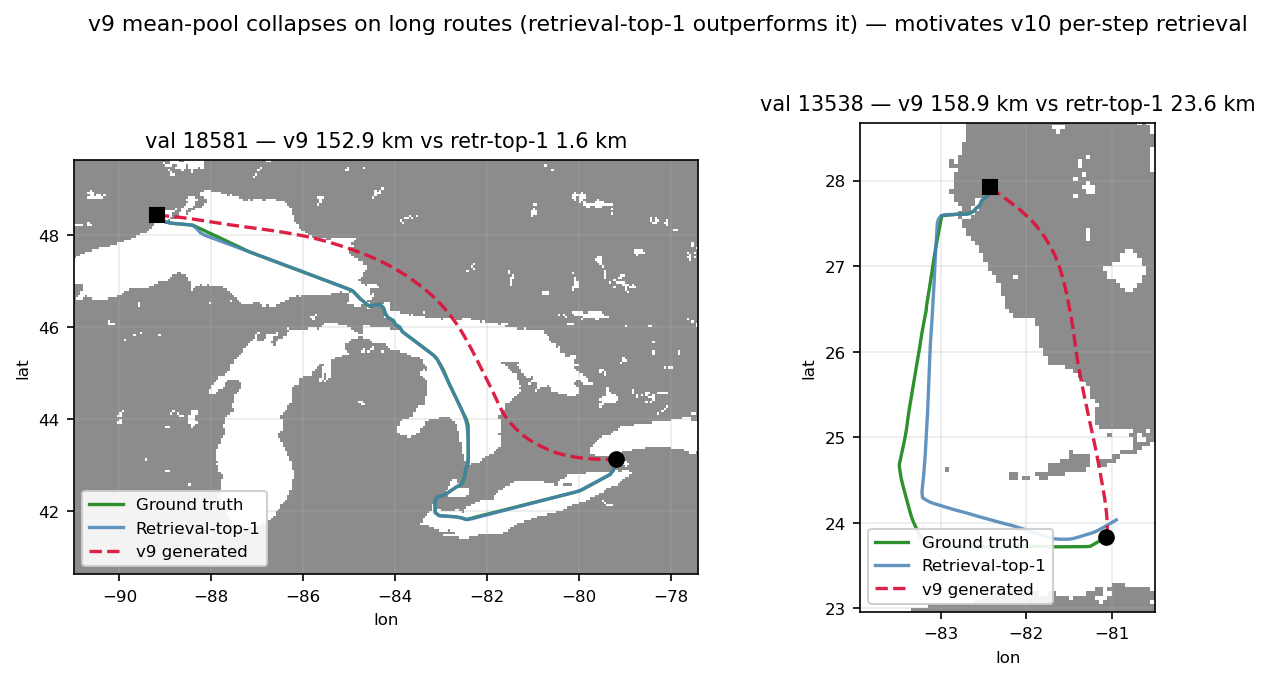
\includegraphics[width=0.95\linewidth]{figures/motiv_v9_long_route_collapse.png}
\caption{Two long-bucket val routes ($>$500\,km) where v9 (red dashed) drifts
         far from ground truth (green), while the zero-training
         retrieval-top-1 neighbour (steelblue) tracks GT closely.
         Mean-pool collapse: v9 has the same five retrieved tokens that
         produced the steelblue route, but those tokens have been compressed
         to centroids before the decoder cross-attends to them.
         This motivates v10's per-step retrieval bank.}
\label{fig:motiv-v9-long}
\end{figure}

\noindent\textit{Training-duration note.}
\texttt{trajgen\_v9\_retrieval} ran for 42/60 epochs.
The architectural-bottleneck conclusion (long-route ADE 7$\times$ short-route
ADE; retrieval-top-1 winning the long bucket) was already firmly visible by
epoch~38; the remaining epochs were dropped to free compute for v10
(whose architectural fix targets the same bottleneck).
Epoch~38 is the checkpoint reported in Table~\ref{tab:v9}.

\subsection{v10 -- Per-timestep retrieval and land-aware training}
\label{sec:v10}

v10 makes three targeted changes to v9, implemented in
\texttt{src/model\_gen\_v10.py}.

\subsubsection{Change 1: Per-step retrieval bank}

\texttt{MeanPoolRouteEncoder} is replaced with \texttt{PerStepRouteEncoder}.
Each retrieved route is subsampled from $T=128$ to $t_\text{retr}=32$ points by
uniform index linspace, projected per-point through a linear layer to
$d_\text{model}$, and augmented with two learned embeddings: a
\emph{route-index embedding} (distinguishing retrieved routes 1--5) and a
\emph{step-index embedding} (distinguishing steps 0--31).
Encoder memory grows from 8 tokens (v9) to $3 + 5 \times 32 = \mathbf{163}$ tokens.
The decoder can now cross-attend to ``neighbour~$k$ at step~$t$'' directly, preserving
per-step route shape.

\begin{figure}[ht]
\centering
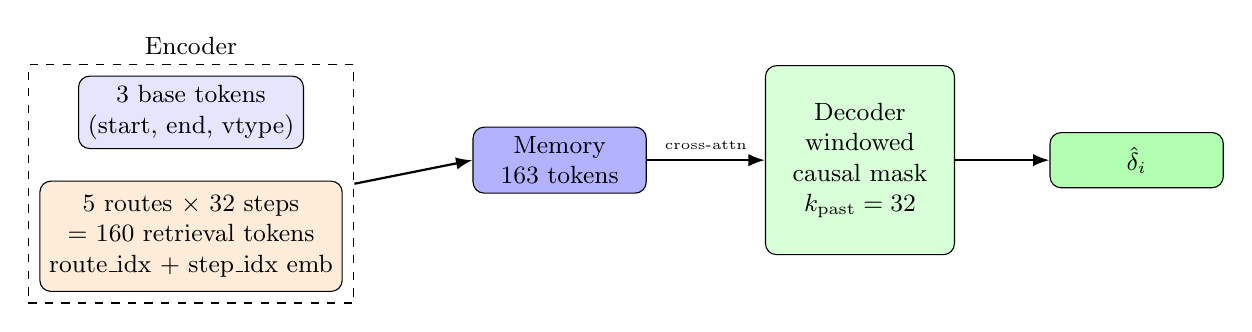
\begin{tikzpicture}[
    node distance=0.6cm and 1.4cm,
    box/.style={draw, rounded corners, minimum width=2.2cm, minimum height=0.7cm,
                align=center, font=\small},
    arr/.style={-{Latex[scale=0.9]}, thick},
  ]
  \node[box, fill=blue!10]  (base) {3 base tokens\\(start, end, vtype)};
  \node[box, fill=orange!15, below=0.4cm of base, minimum width=2.2cm,
        minimum height=1.4cm]
    (retr) {5 routes $\times$ 32 steps\\= 160 retrieval tokens\\route\_idx + step\_idx emb};
  \node[draw, dashed, fit=(base)(retr), inner sep=4pt, label=above:{\small Encoder}]
    (encbox) {};
  \node[box, fill=blue!30, right=1.5cm of encbox, yshift=0.3cm]
    (mem) {Memory\\163 tokens};
  \node[box, fill=green!15, right=1.5cm of mem, minimum height=2.4cm,
        minimum width=2.4cm] (dec) {Decoder\\windowed\\causal mask\\$k_\text{past}=32$};
  \node[box, fill=green!30, right=1.2cm of dec] (out) {$\hat\delta_i$};

  \draw[arr] (encbox.east) -- (mem.west);
  \draw[arr] (mem.east) -- (dec.west) node[midway,above,font=\tiny]{cross-attn};
  \draw[arr] (dec.east) -- (out.west);
\end{tikzpicture}
\caption{v10 encoder-decoder.  The 163-token memory bank exposes per-step shape from
         each of the 5 retrieved routes, replacing v9's mean-pool collapse.
         The windowed causal mask (k\_past\,=\,32) limits self-attention drift over
         the 128-step rollout.}
\label{fig:v10-arch}
\end{figure}

\subsubsection{Change 2: Windowed causal mask}

A windowed causal mask blocks attention to steps further than $k_\text{past}=32$
in the decoder's own past:
\[
  M_{ij} = \begin{cases}
    0      & \text{if } j \le i \text{ and } j \ge i - k_\text{past} \\
    -\infty & \text{otherwise.}
  \end{cases}
\]
This limits drift from stale self-state over 128 autoregressive steps.

\subsubsection{Change 3: Land-aware loss and hard-projection inference}
\label{sec:land-sdf}

A differentiable land loss is added to Eq.~\eqref{eq:gen-loss}:
\begin{equation}
  \mathcal{L}_\text{land} = \frac{1}{T}\sum_i \text{ReLU}\!\left(\text{sdf\_km}(x_i^\text{raw}) - 10\right)^2,
  \label{eq:land-loss}
\end{equation}
where $\text{sdf\_km}$ is sampled bilinearly from the precomputed $0.05^\circ$ SDF
raster (Figure~\ref{fig:land-sdf}).
The threshold 10\,km discounts rasterisation noise: the GT data in
\texttt{trajgen\_128.npz} itself has 10.83\,\% land fraction at 10\,km,
purely from GSHHS polygon clipping artefacts.
The coefficient $\lambda_\text{land} = 0.01$ was chosen to keep the land gradient
comparable to $\mathcal{L}_\delta$ without destabilising early training.

The full v10 loss is:
\[
  \mathcal{L}_{v10} = \mathcal{L}_\delta
                    + 10\,\mathcal{L}_\text{endpoint}
                    + 1\,\mathcal{L}_\text{smooth}
                    + 0.01\,\mathcal{L}_\text{land}.
\]

\textbf{Differentiable SDF sampling.}
PyTorch's \texttt{F.grid\_sample} backward is unimplemented on Apple Silicon MPS.
A platform-independent bilinear sampler was therefore hand-rolled in
\texttt{src/land\_mask.py}:
integer cell indices are detached (no gradient); floating-point offsets
$(f_r, f_c)$ carry the gradient through a manual bilinear combination:
\[
  v \approx (1-f_r)(1-f_c)\,v[r,c]
           + (1-f_r) f_c\,v[r,c{+}1]
           + f_r(1-f_c)\,v[r{+}1,c]
           + f_r f_c\,v[r{+}1,c{+}1].
\]

\textbf{Hard-projection at inference.}
After each decoder step, if $\text{sdf\_km}(\text{pos}) > 10$, the position is
projected to the nearest water cell via breadth-first search (BFS) in
\texttt{LandMask.project\_to\_water} (20-cell search radius $\approx$ 100\,km).
The projected point is fed back into the decoder for the next step.
After rollout, linear endpoint correction is applied; corrected points with
$\text{sdf} > 10$ are re-projected.

\begin{figure}[ht]
\centering
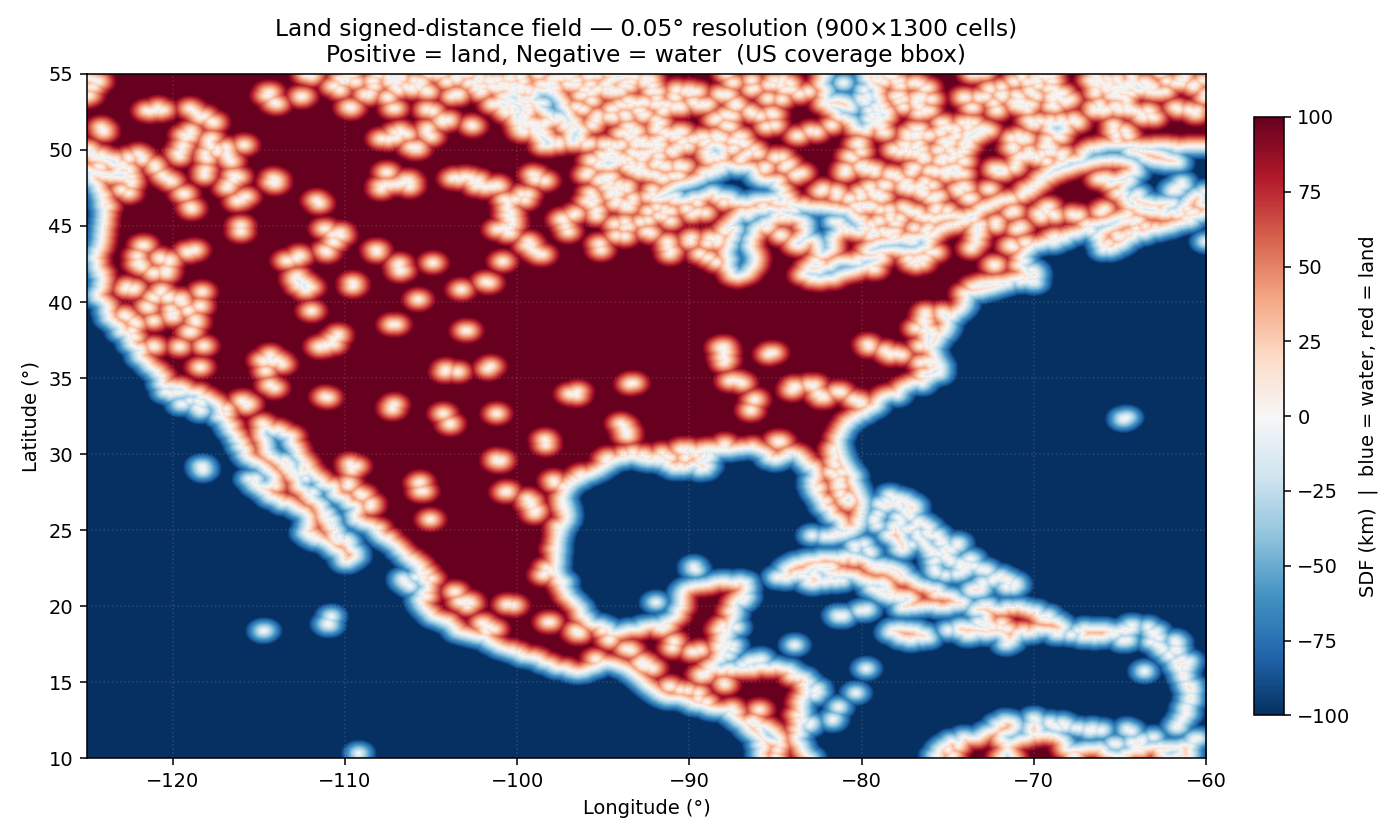
\includegraphics[width=0.85\linewidth]{figures/land_sdf.png}
\caption{Land SDF raster at $0.05^\circ$ ($\approx5\,km$) resolution over
         the US coverage bbox.
         Blue = water (negative SDF), red = land (positive SDF).
         Saturated at $\pm100\,km$ for visual clarity.}
\label{fig:land-sdf}
\end{figure}

\subsubsection{Results on dirty data}

\begin{table}[ht]
\centering
\caption{v10 variants on dirty \texttt{trajgen\_128.npz} ($n=500$, seed=42).}
\label{tab:v10-dirty}
\begin{tabular}{lrrc}
\toprule
Configuration & \ade{} (m) & land\%@10km & cross\%@0km \\
\midrule
v10 raw                     & 6584  & 7.15 & 36.2 \\
v10 + hard-projection       & 9345  & 0.02 & 0.4  \\
v10 + WaterRouter snap-only & 7934  & 0.09 & 1.2  \\
Retrieval-top-1             & 6470  & 11.03 & 35.6 \\
Great-circle                & 8226  & 13.47 & 41.8 \\
\bottomrule
\end{tabular}
\end{table}

Hard-projection drove land-crossing to near zero but incurred $+42$\,\% \ade{}.
The WaterRouter snap-only post-processor (Section~\ref{sec:water-router}) reduced this
penalty to $+20$\,\%; the root cause of both penalties---ground-truth data quality---
is addressed in Section~\ref{sec:e1}.

Figure~\ref{fig:motiv-v10-router} shows what ``v10 raw still leaks land''
looks like on two val examples, alongside the same prediction after
WaterRouter snap-only.
The raw outputs cut across small islands and short land bridges;
the post-processor pushes each offending waypoint back to the nearest
connected water cell.
This is the qualitative justification for keeping a water-validity layer
on top of the land-aware loss, even though the loss already discourages
crossings on average.

\begin{figure}[ht]
\centering
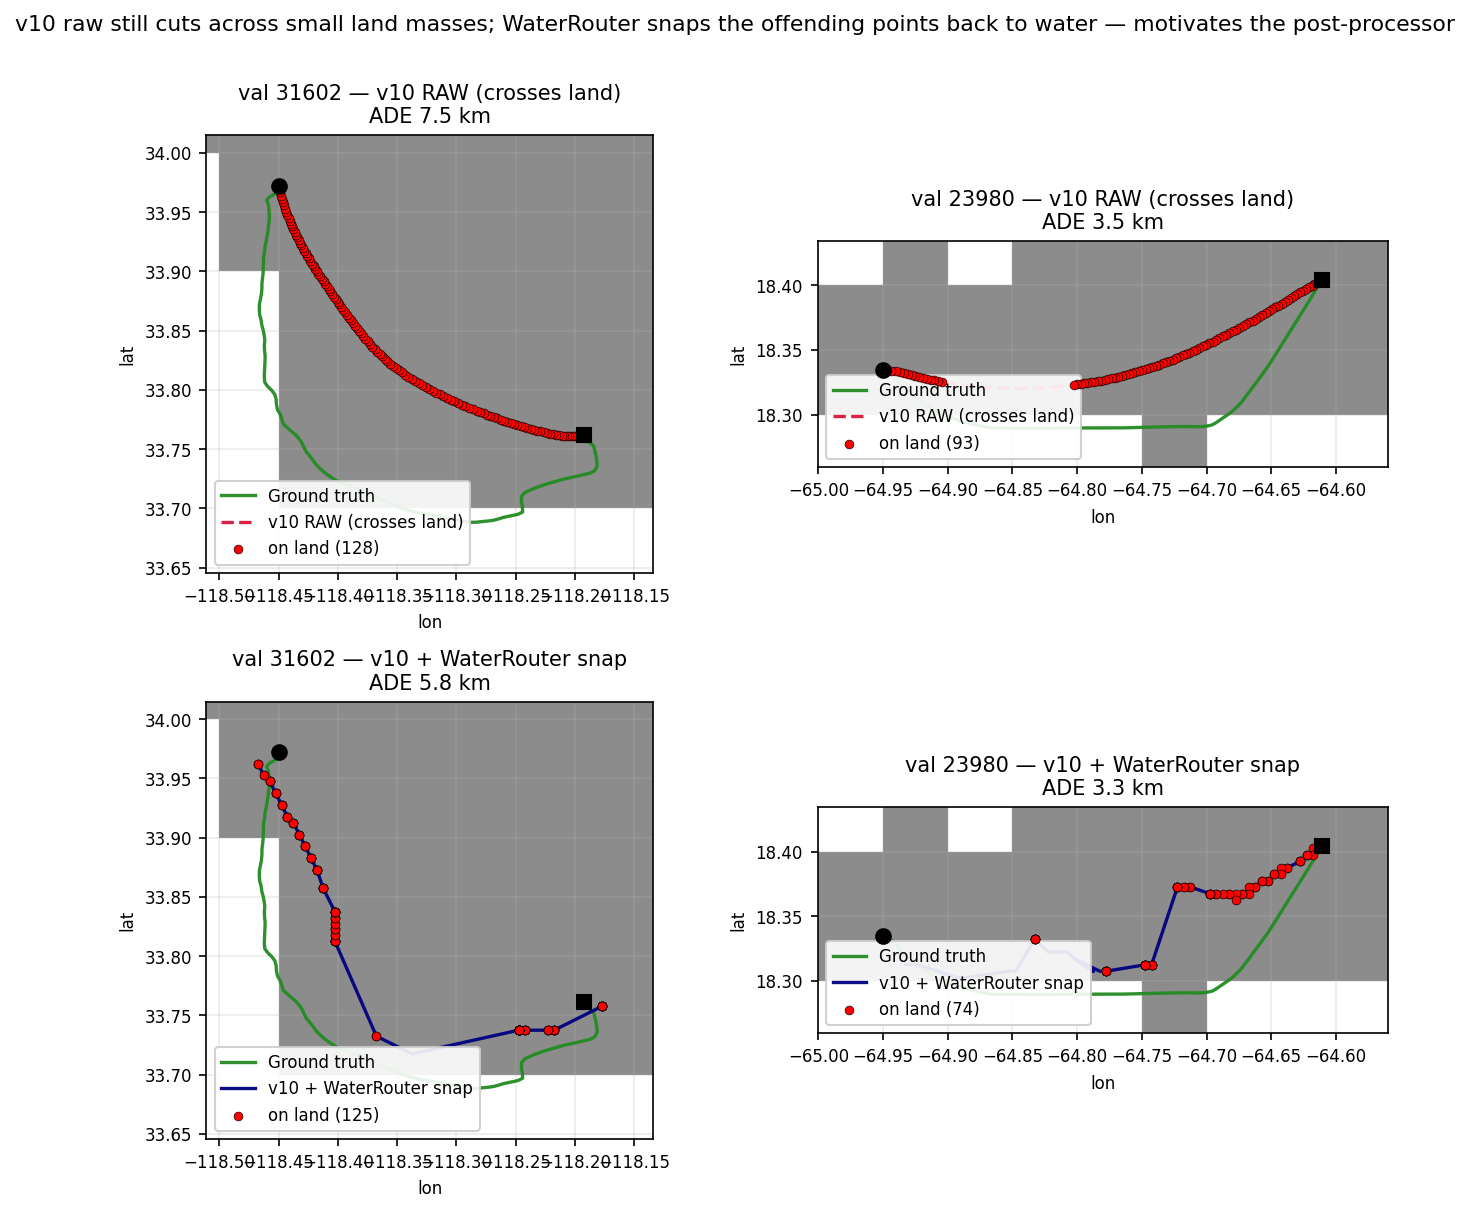
\includegraphics[width=0.95\linewidth]{figures/motiv_v10_raw_crosses_land.png}
\caption{Two val routes where v10 raw output (top row, red dashed) crosses
         small land features that the differentiable land loss did not
         eliminate.  Grey blocks are land masses (rasterised GSHHS coastline);
         white is water; green is the ground-truth route, red dashed is the
         v10 raw prediction, and navy solid (bottom row) is the same trajectory
         after WaterRouter snap-only --- every offending waypoint moved to the
         nearest connected water cell on the $0.005^\circ$ graph.
         The ADE penalty on dirty data is the price of also moving
         many \emph{borderline} (coastal-river) waypoints; on clean data
         (Section~\ref{sec:e1}, Table~\ref{tab:e1}) the penalty essentially
         vanishes because few waypoints need snapping.}
\label{fig:motiv-v10-router}
\end{figure}

\noindent\textit{Training-duration note (v10).}
\texttt{trajgen\_v10} ran for 52/60 epochs.  Training was halted once the
val curves (Figure~\ref{fig:training-curves}) plateaued and the
land-crossing rate on the val set settled below 8\,\% --- additional
epochs would not change the ``raw v10 leaks land'' picture that the
WaterRouter is built to repair.  Epoch~52 is the production checkpoint
quoted as ``v10 ep52'' throughout this report.

\subsection{WaterRouter post-processor}
\label{sec:water-router}

The WaterRouter (\texttt{src/water\_router.py}) is a non-learned post-processor
that snaps v10 raw waypoints to water without retraining.

\textbf{Fine-resolution graph.}
\texttt{scripts/data/build\_water\_graph.py} builds a $0.005^\circ$ ($\approx0.5\,km$)
graph from the same GSHHS polygons.
Each water cell carries a \texttt{neighbor\_bits} mask encoding which of its
8 neighbours are also water.
File size: $\approx$117\,MB for the US bbox.

\textbf{Snap-only mode (production).}
For each waypoint with $\text{sdf} > 10$:
find the nearest fine-grid water cell satisfying (a) $\text{neighbor\_bits} > 0$
(not a landlocked inlet artefact) and (b) coarse-SDF below threshold.
Condition (a) prevents snapping to isolated one-pixel water artefacts with no
path to the open ocean.

\begin{algorithm}[ht]
\caption{WaterRouter Snap-Only}
\label{alg:snap}
\begin{algorithmic}[1]
\REQUIRE trajectory $\mathbf{x}$ (128 waypoints), coarse SDF, fine-grid water graph
\FOR{$i = 1$ \textbf{to} $128$}
  \IF{$\text{sdf\_coarse}(x_i) > 10$}
    \STATE $c \gets$ fine-grid cell nearest to $x_i$
    \STATE BFS from $c$: find nearest $c'$ with $\text{neighbor\_bits}(c') > 0$
            AND $\text{sdf\_coarse}(c') \le 10$
    \STATE $x_i \gets \text{centre}(c')$
  \ENDIF
\ENDFOR
\STATE \RETURN $\mathbf{x}$
\end{algorithmic}
\end{algorithm}

Latency: $\approx22\,ms$ per trajectory on a single CPU core.
The bridging mode (\texttt{do\_segment\_bridge=True}), which uses A* search to
re-route segments crossing land, was found to hurt \ade{} more than it fixed
residual crossings and is disabled in production.

\subsection{E1 -- Upstream data cleaning}
\label{sec:e1}

\subsubsection{Diagnosis}

Figure~\ref{fig:motiv-dirty-gt} shows two examples of what the
``dirty'' ground-truth data looks like: two AIS tracks from
\texttt{trajgen\_128.npz} whose pings sit mostly on inland water --- rivers,
estuaries, and harbour channels not represented in the GSHHS coarse coastline.
These are not modelling artefacts; they are the supervisory targets that
trained every v1--v9 model in this report.

\begin{figure}[ht]
\centering
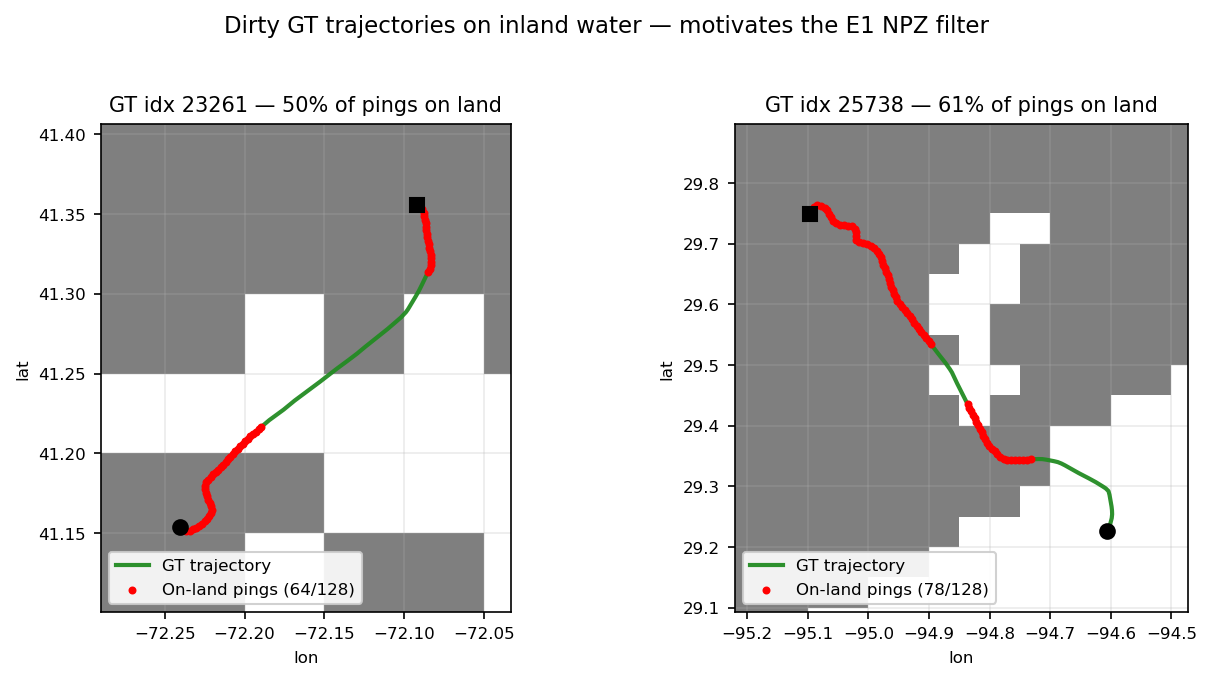
\includegraphics[width=0.95\linewidth]{figures/motiv_dirty_gt_on_river.png}
\caption{Two ground-truth trajectories from \texttt{trajgen\_128.npz} that
         sit on inland water (rivers, harbour channels).
         Land is shaded grey, red dots flag GT pings whose
         coarse-SDF says ``land''.
         These trajectories are valid AIS recordings but live in waters that
         the $0.05^\circ$ GSHHS-derived coastline does not represent,
         and they constitute roughly 10\,\% of all pings in the raw NPZ.
         Training any model that should ``not cross land'' on data like this
         is asking it to learn the opposite of its supervisory targets;
         the E1 filter (next subsection) removes them.}
\label{fig:motiv-dirty-gt}
\end{figure}

Running \texttt{scripts/eval/land\_crossing\_diagnostic.py} on the \emph{ground truth}
trajectories in \texttt{trajgen\_128.npz} returned:
$\text{land\%@10km} = 10.83$\,\%,
$\text{cross\%@10km} = 36.0$\,\%,
$\text{cross\%@0km} = 87.6$\,\%.
The data itself was crossing land; the model trained on it was being asked to learn
``do not cross land'' while 36\,\% of its supervisory targets did exactly that.

\subsubsection{The filter}

\texttt{scripts/data/filter\_trajgen\_npz.py} retains only tracks satisfying:
\[
  \text{land5\_frac} \le 0.02
  \quad\text{AND}\quad
  \max_i \text{sdf\_km}(x_i) \le 10,
\]
where \texttt{land5\_frac} is the fraction of waypoints with $\text{sdf} > 5$~km.
The output, \texttt{trajgen\_128\_clean.npz}, contains 61,024 of the original
207,000 tracks (29.4\,\%).

\subsubsection{Impact}

\begin{table}[ht]
\centering
\caption{v10 ep52 weights re-evaluated on clean vs.\ dirty data.}
\label{tab:e1}
\begin{tabular}{lrrr}
\toprule
Metric & Dirty data & Clean data & Change \\
\midrule
GT land\%@10km       & 10.83 & \textbf{0.00}  & $-100$\,\% \\
v10 raw \ade{} (m)   & 6584  & \textbf{6278}  & $-4.6$\,\% \\
v10 + hard-proj \ade{} & 9345 & \textbf{6579} & $-30$\,\% \\
v10 + WaterRouter \ade{} & 7934 & \textbf{6282} & $-21$\,\% \\
v10 + WaterRouter cross\%@10km & 1.2 & \textbf{0.0} & $-100$\,\% \\
Retr-top-1 \ade{}    & 6470  & 12373           & $+91$\,\%  \\
\bottomrule
\end{tabular}
\end{table}

The water-strict \ade{} penalty from snap-only essentially vanished on clean data
(6282~m vs.\ 6278~m v10 raw on the same slice) because almost no waypoints needed
snapping.
The retrieval-top-1 regression on clean data is expected: the corpus shrank by 70\,\%
and long-bucket sample count grew from 7 to 23, making KNN matches sparser.

\textbf{The lesson}: E1 establishes that the train/test distribution shift
induced by the dirty corpus was responsible for a substantial fraction of
v10's water-strict \ade{} cost.  Data cleaning is therefore best understood
as a \emph{prerequisite} for fair architectural evaluation --- it removes
confounding training-set artefacts (38\,\% land-crossing in the ground truth
itself) that would otherwise mask the contribution of v10's per-timestep
retrieval and land-aware loss.

\subsection{v11 -- Halton-cone pointer (parked)}
\label{sec:v11}

v11 replaced continuous displacement regression with a discrete pointer over
a per-step candidate pool of water-only positions.
Candidates were drawn by Halton quasi-random sampling~\cite{halton1960quasi}
within a $[3\,km, 25\,km]$ forward cone aligned with bearing-to-destination.
The model selected the best candidate via a masked softmax pointer head
(\texttt{src/model\_gen\_v11.py}).

\textbf{Result}: \ade{} = 30000\,m, path-length ratio $13\times$.
\textbf{Diagnosis}: the median GT step after arc-length resampling to 128 points is
0.34\,km; the cone minimum radius (3\,km) was $9\times$ larger.
The model could only pick the smallest available candidate at every step---and even
that overshot by almost an order of magnitude.
\textbf{Lesson}: a candidate pool must be calibrated to the empirical step-size
distribution of the training data, not to intuitions about ``reasonable'' step sizes.
v11 is parked.

\noindent\textit{Training-duration note.}
\texttt{trajgen\_v11\_lite} ran its full 40/40 epochs.  The failure is
structural (step-size mismatch), not under-training; further epochs would
not change \ade{}.

\subsection{v12 -- Water-cell K-ring pointer (abandoned)}
\label{sec:v12}

v12 (\texttt{src/model\_gen\_v12.py}) addressed the v11 mismatch by deriving the
candidate pool from the actual water-cell graph.
At each decoder step, candidates are the Chebyshev-$K$ ring of cells around the
current cell plus a learned END token; land cells receive $-\infty$ logit before
softmax, giving a \emph{structural} water guarantee: the model cannot output a
land cell.
A small offset head regresses a continuous $({\Delta}lon, {\Delta}lat)$ within the
chosen cell for sub-km precision.

\begin{table}[ht]
\centering
\caption{v12 failure (40-epoch run, $K=4$, $n=500$, seed=42).}
\label{tab:v12}
\begin{tabular}{lrrrr}
\toprule
 & v9 ep38 & Retr-top-1 & GC & v12 (ep40) \\
\midrule
\ade{} (m)             & 6207  & 6741  & 8539  & \textbf{27365} \\
\fde{} (m)             & 0     & 6160  & 0.1   & 41038 \\
\ade{} long (m)        & 46631 & 22845 & 95900 & 236014 \\
strict-0 cross\%       & ---   & ---   & ---   & 81\,\% \\
\bottomrule
\end{tabular}
\end{table}

\textbf{Three structural failures:}
\begin{enumerate}
  \item \textbf{K\,=\,4 silently drops long transitions.}
        P90/P95/P99 of GT cell transitions at $0.005^\circ$ are 4/5/10 cells.
        Any transition with $|dx|>4$ or $|dy|>4$ maps to
        \texttt{ignore\_index=-100} in cross-entropy, contributing zero gradient.
        The model never learns long jumps; at inference it is forced through
        short ring-steps, producing wandering routes
        (path-length ratio 1.48).
  \item \textbf{CE on cell pointer is uncorrelated with rollout ADE.}
        Top-1 cell accuracy reached 87.2\,\% over 40 epochs while \ade{}
        remained catastrophic.
        $\lambda_\text{ade}=0.001$ contributed
        $\sim 3.6 \times 10^{-5}$ to total loss vs.\ CE contributing $\sim 0.545$
        ($50{-}100\times$ dominant).
        \emph{Auxiliary losses must be calibrated by gradient magnitude, not intuition.}
  \item \textbf{Argmax rollout drifts laterally.}
        Greedy argmax selection over 128 steps accumulates lateral offset that
        linear endpoint correction cannot undo.
\end{enumerate}

v12 is abandoned; the post-mortem lives in \texttt{docs/decisions.md\#v12}.

\noindent\textit{Training-duration note.}
\texttt{trajgen\_v12} ran its full 40/40 epochs.  Top-1 cell accuracy
reached 87.2\,\% at the final epoch while \ade{} stayed
4.4$\times$ worse than v9 throughout --- this is the per-step / rollout
disconnect (Section~\ref{sec:contributions}, central negative finding)
playing out a second time.  The full schedule was run precisely to rule out
``maybe more training would fix it''; it did not.

Figure~\ref{fig:motiv-v12-zigzag} shows what v12's output looks like in
practice: predicted trajectories trace short, axis-aligned cell-to-cell
moves and accumulate lateral drift over the 128-step rollout.  The
$K{=}4$ ring (the second-failure column in the post-mortem above) prevents
the larger diagonal jumps that real GT routes make; greedy argmax then
chooses whichever ring cell is roughly toward the destination, producing
the Manhattan zigzag visible in every panel.

\begin{figure}[ht]
\centering
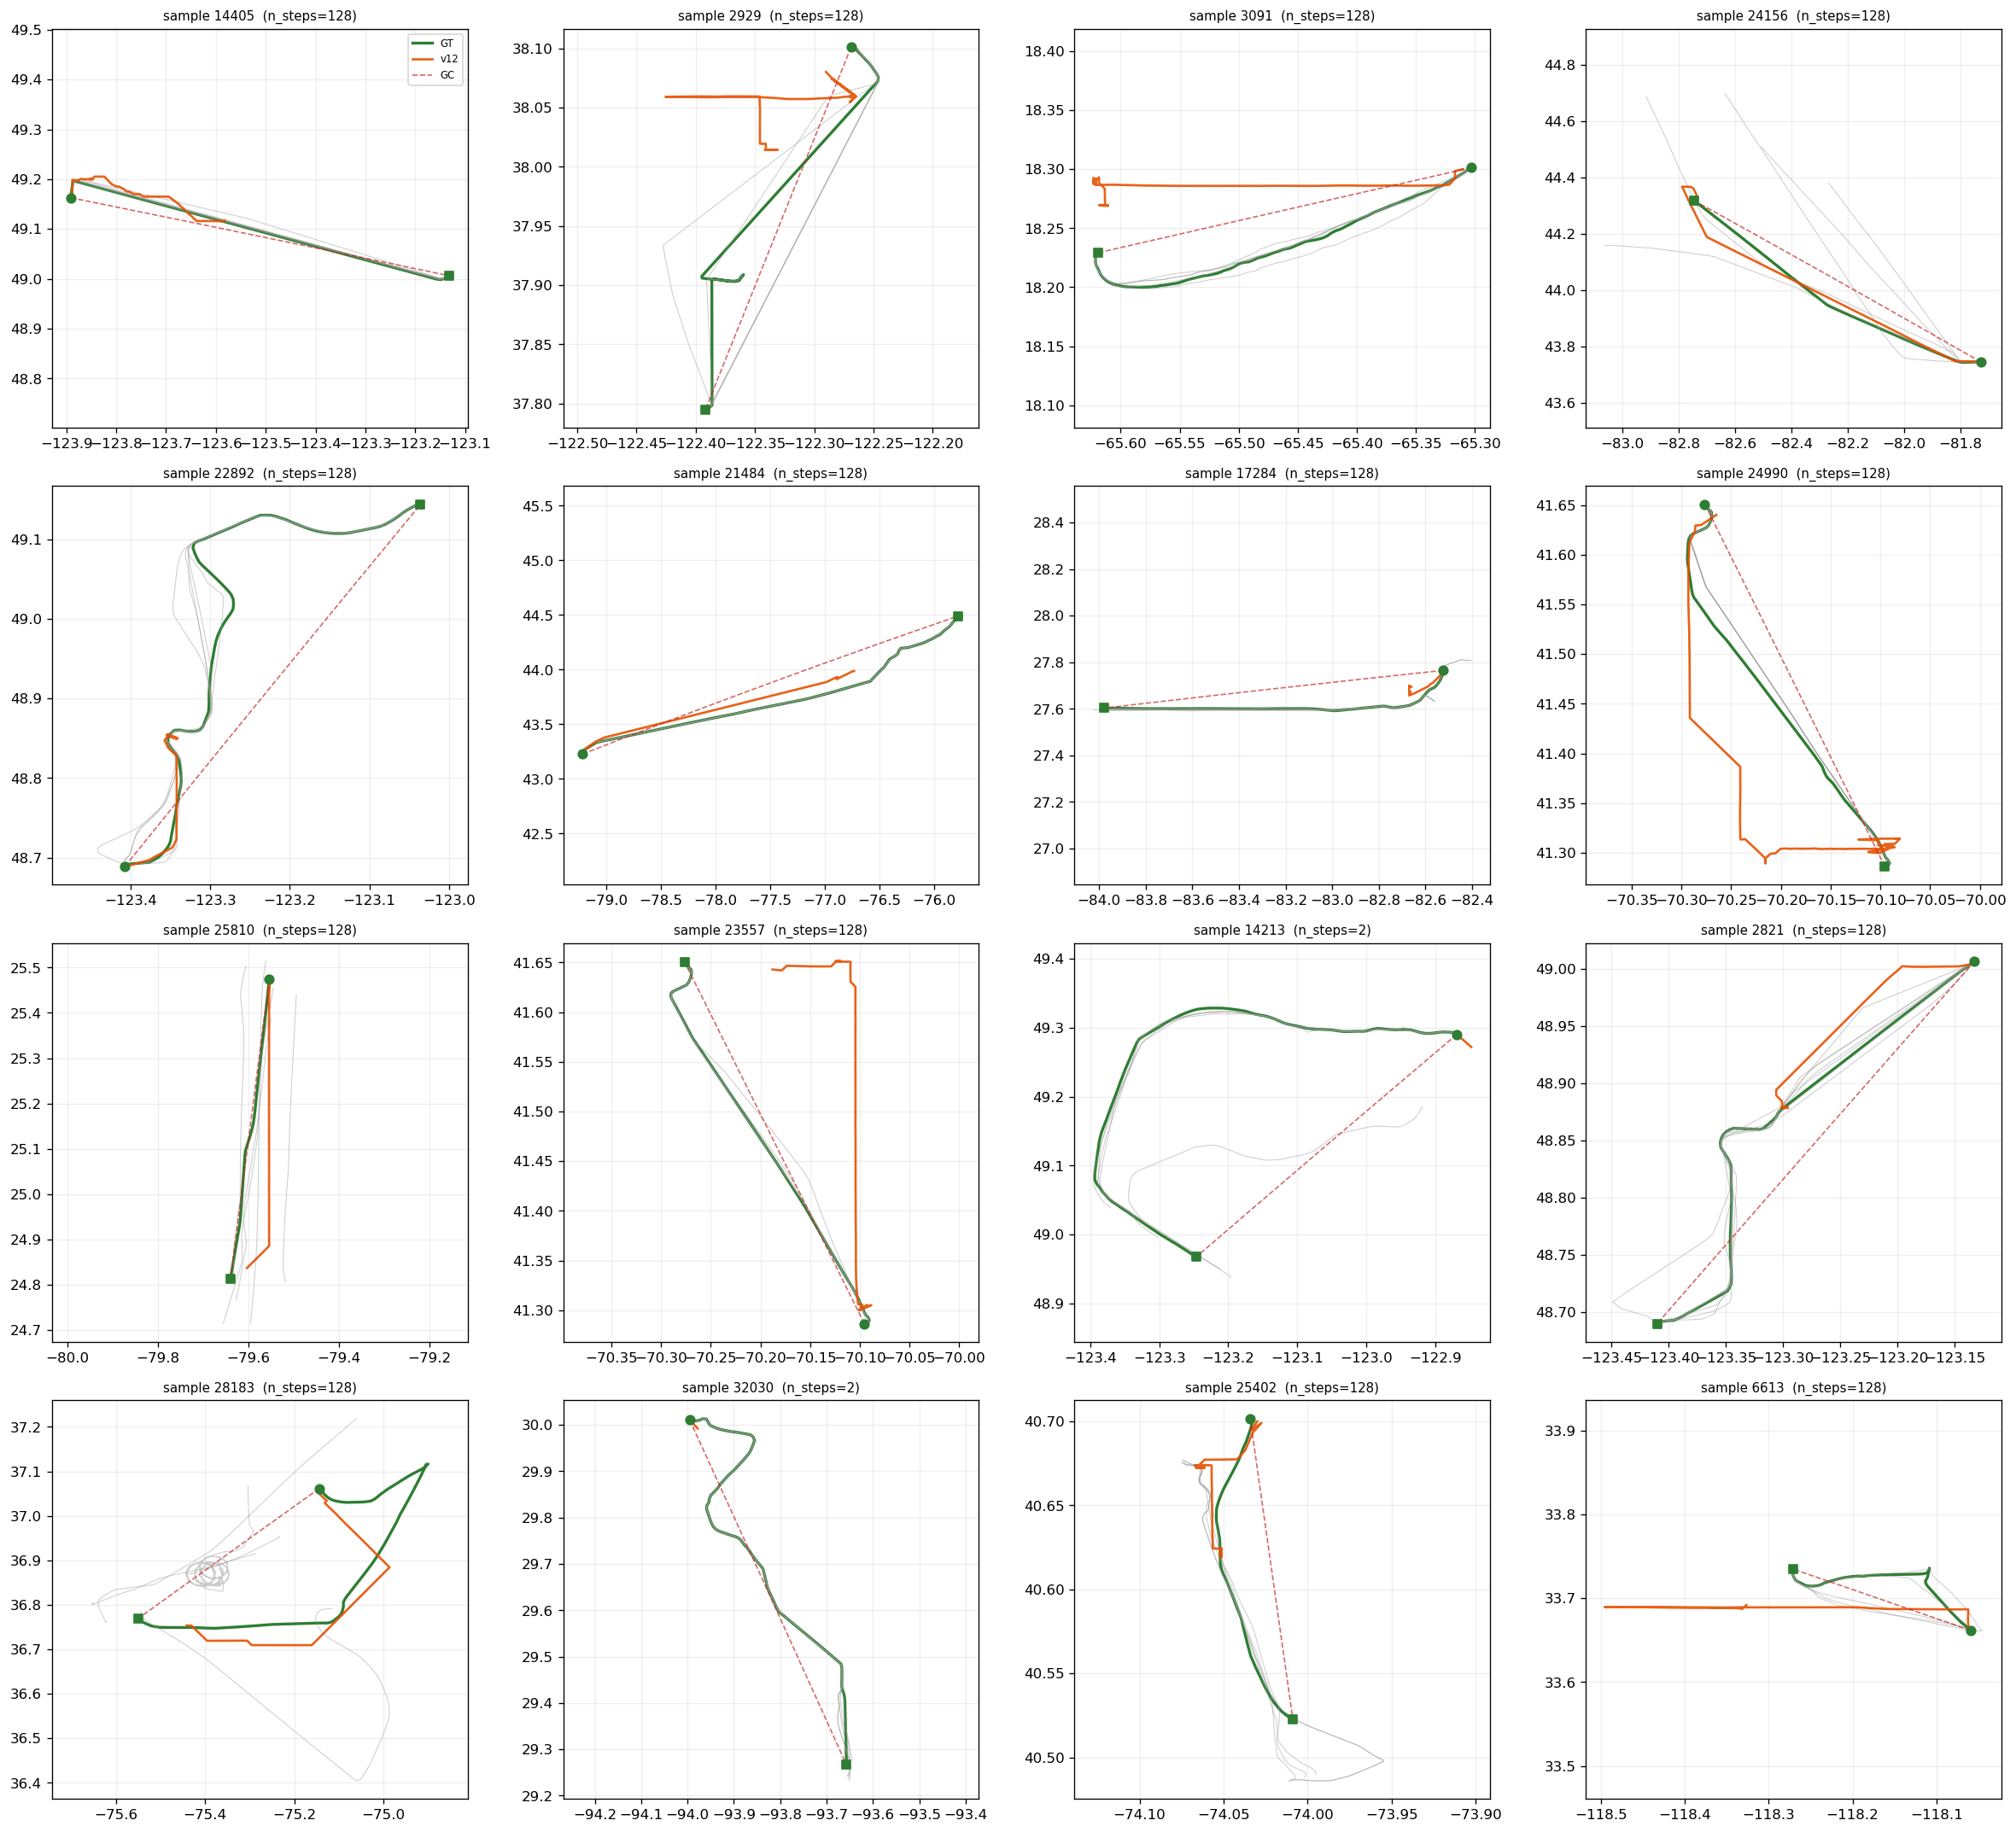
\includegraphics[width=0.92\linewidth]{figures/motiv_v12_zigzag.png}
\caption{v12 cell-pointer output on a grid of val routes (this is the same
         \texttt{viz\_v12.png} qualitative panel from
         \texttt{scripts/eval/visualize\_gen\_v12.py}).
         Green = GT, blue = retrieved neighbours, red dashed = v12 prediction.
         The characteristic axis-aligned zigzag is structural: the
         K-ring candidate set is mostly cardinal-direction neighbours,
         and 128 sequential argmax picks compound into wandering routes
         with path-length ratio 1.48.}
\label{fig:motiv-v12-zigzag}
\end{figure}

\begin{figure}[ht]
\centering
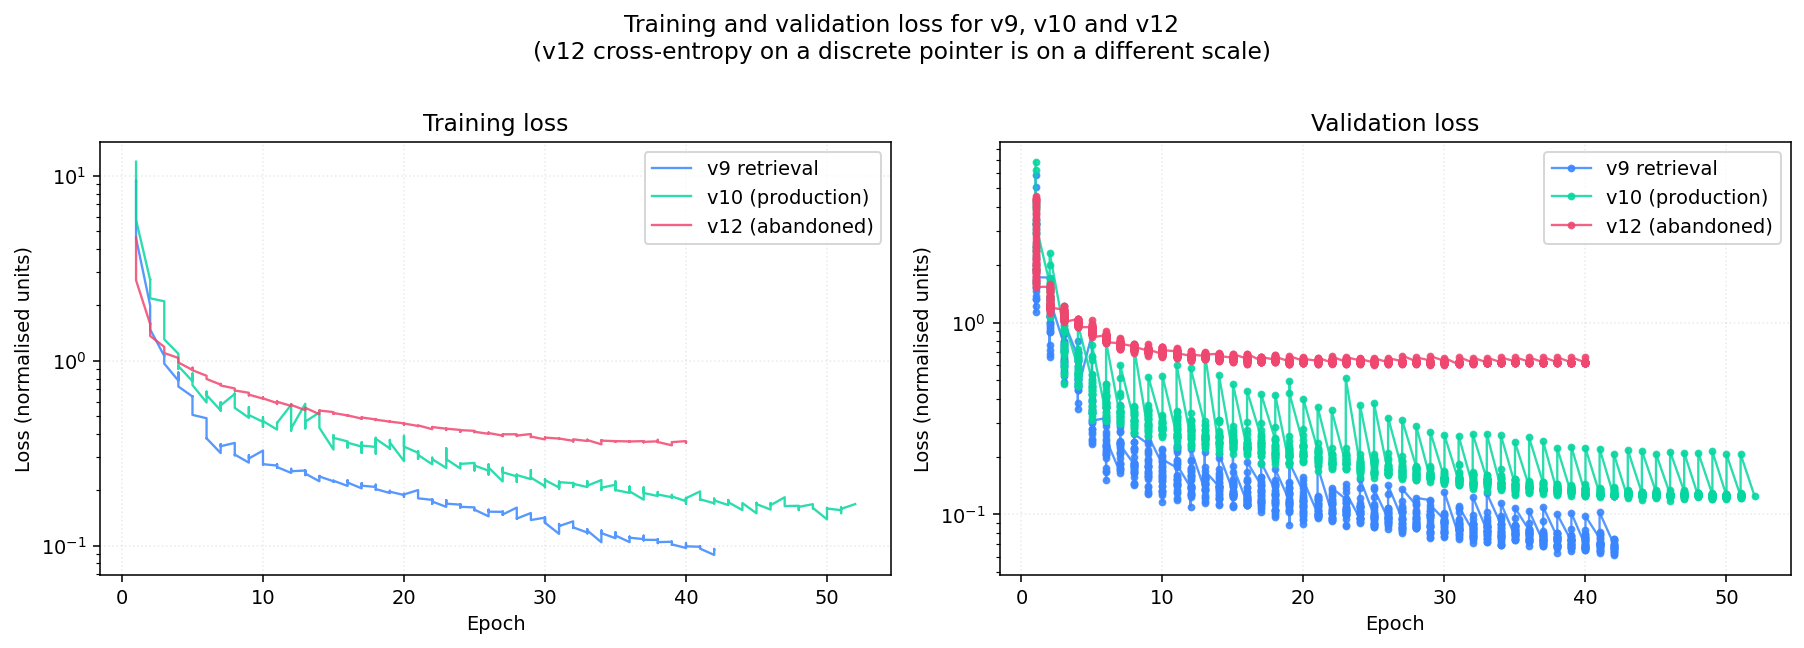
\includegraphics[width=\linewidth]{figures/v9_v10_v12_training_curves.png}
\caption{Training and validation loss for v9 (retrieval), v10 (production), and v12
         (abandoned) on log scale.
         Note that v12's CE loss is on a fundamentally different scale and not
         comparable to v9/v10's regression loss.}
\label{fig:training-curves}
\end{figure}

% =====================================================================
\section{Results and Discussion}
\label{sec:results}

\subsection{Summary of all trajectory-generation experiments}

Figure~\ref{fig:ade-by-model} provides a visual overview of \ade{} across all
trajectory-generation model versions.
With linear endpoint correction, all trained \ade{}-target models reach
\fde{}~$\approx 0$ by construction; the \fde{} discriminator is meaningful
only for retrieval-top-1 (\fde{} = 5603\,m, no correction applied) and for
v10\,+\,WaterRouter (small non-zero offset from snapping at the final
waypoint).

\begin{figure}[ht]
\centering
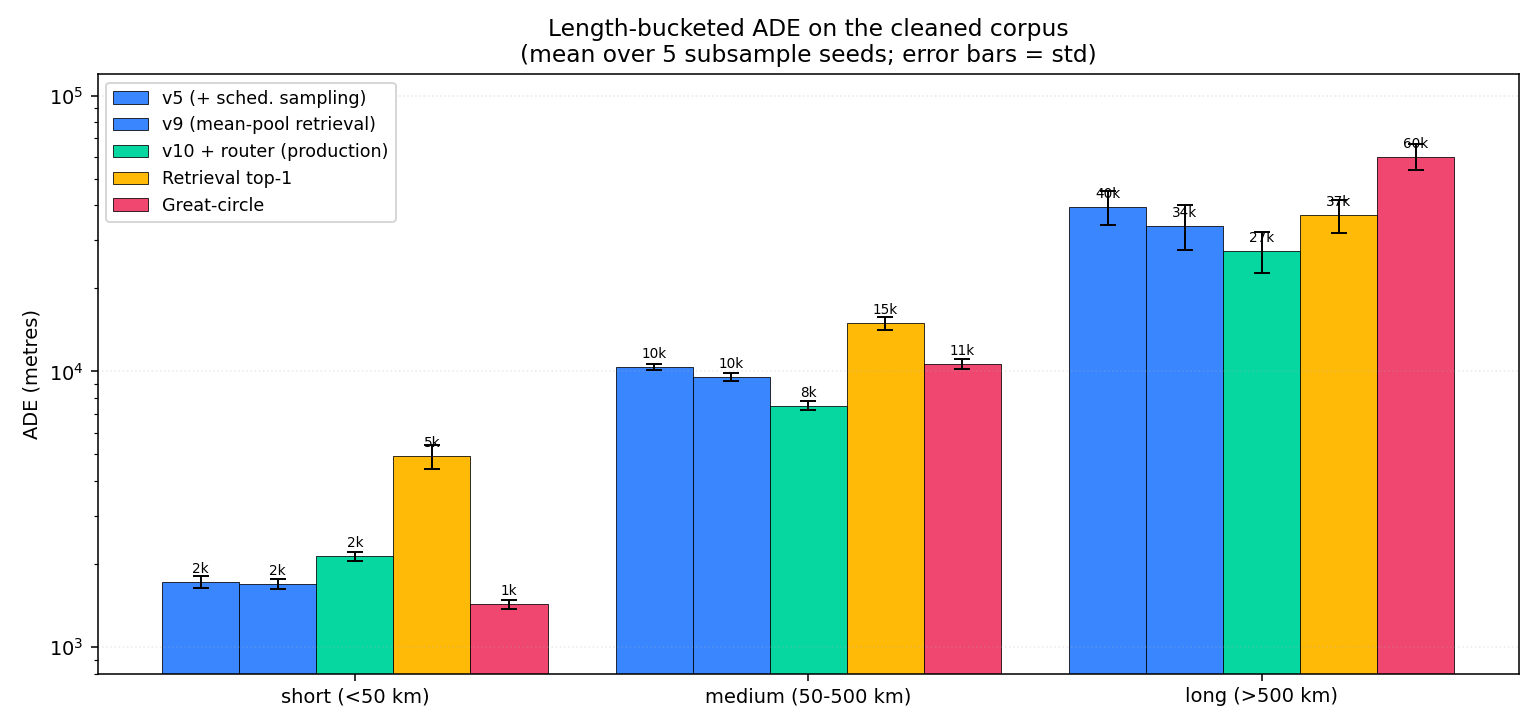
\includegraphics[width=\linewidth]{figures/length_bucketed_ade.png}
\caption{Length-bucketed ADE (log scale).
         v9 wins short and medium; retrieval-top-1 dominates the long-tail ($>$500\,km).
         No single model wins all three buckets --- the key motivation for v13's
         length router.}
\label{fig:length-bucketed}
\end{figure}

\subsection{Cross-cutting findings}

\begin{enumerate}

\item \textbf{Per-step validation loss is uncorrelated with rollout ADE.}
      The architectural ladder v2$\to$v5 improved val\_delta by 14\,\% (0.086 $\to$ 0.074)
      with zero real-world ADE improvement.
      The same pattern appeared in v12: CE top-1 accuracy reached 87.2\,\% while
      \ade{} was 4.4$\times$ v9.
      Only end-to-end rollout evaluation is informative.

\item \textbf{Retrieval was the only intervention that produced a clear
      \ade{} drop over the baseline.}
      A zero-training, positions-only retrieval-top-1 baseline
      (5-D KNN over start/end with no vessel-type weighting, used as the
      v9 design gate) achieved \ade{} = 5489\,m,
      18.7\,\% lower than v5's 6753\,m on the same \texttt{seed=42} subsample
      (\texttt{results/summary.csv}, row \texttt{retrieval\_baseline\_top1}).
      Once vessel-type weighting was added (the configuration used for the v9
      training comparison in Section~\ref{sec:v9}), retrieval-top-1 measured
      6470\,m and v9 reached 6207\,m, a $\sim$4\,\% reduction over that
      retrieval baseline.
      All other architectural elaborations in the v2--v5 ladder
      (bigger model, bearing features, scheduled sampling) and in v10
      (land loss, windowed mask) produced no \ade{} change larger than the
      $\sim$225\,m subsample-noise floor measured in
      Appendix~\ref{app:variance}.
      Because no multiple-training-seed variance was measured for v5, v9, or
      v10, the report cannot rule out the possibility that the v9-over-v5 gap
      partially reflects training-seed luck rather than architecture; the
      $\sim$19\,\% retrieval-vs-v5 gap, however, is large enough relative to
      the subsample noise floor that this caveat is unlikely to invert the
      finding.

\item \textbf{Data quality dominates model quality.}
      Filtering the training set (E1, Section~\ref{sec:e1}) reduced the water-strict
      \ade{} by 21\,\% --- larger than any model change.
      The land-crossing penalty from hard-projection collapsed from $+42$\,\% to
      $+5$\,\% after cleaning.

\item \textbf{Constraint losses need constraint-violating examples.}
      Both the obstacle loss (v6/v7) and the land loss (v10) require training
      examples where the constraint \emph{would} be violated to generate
      a non-zero gradient.
      The obstacle loss never fired structurally; the land loss fired inconsistently
      on dirty data (threshold too close to GT's own land rate).

\item \textbf{Structural guarantees are decoupled from trajectory quality.}
      v12's masked-logit pointer guaranteed $\text{cross\%@0} = 81$\,\% --- better
      than its own ground truth (87\,\%) --- while producing \ade{} 4.4$\times$
      worse than v9.
      Water-validity and route accuracy are distinct objectives requiring separate
      engineering.

\end{enumerate}

\subsection{Production system use-case ranking}
\label{sec:ranking}

\begin{table}[ht]
\centering
\caption{Use-case ranking for the production system.}
\label{tab:ranking}
\begin{tabular}{llrr}
\toprule
Use case & Configuration & \ade{} (m) & land\%@10km \\
\midrule
Water-strict deployment  & v10+router, clean data    & \textbf{6282} & \textbf{0.00} \\
Best \ade{}, no constraint & v9 ep38, dirty data     & \textbf{6207} & 12.81 \\
Best long-route ($>$500\,km) & Retr-top-1, dirty & 18785\textsuperscript{*} & 11.03 \\
Geometric baseline       & Great-circle              & 8226          & 13.47 \\
\bottomrule
\end{tabular}
\vspace{0.5em}
\small\textsuperscript{*}Long bucket only ($n=7$); overall retr-top-1 ADE is 6470\,m.
\end{table}

The production system has no single model that simultaneously achieves lowest
overall \ade{}, lowest long-bucket \ade{}, and strict water-validity.
This three-way trade-off is the primary motivation for the v13 design in
Section~\ref{sec:future}.

\begin{figure}[ht]
\centering
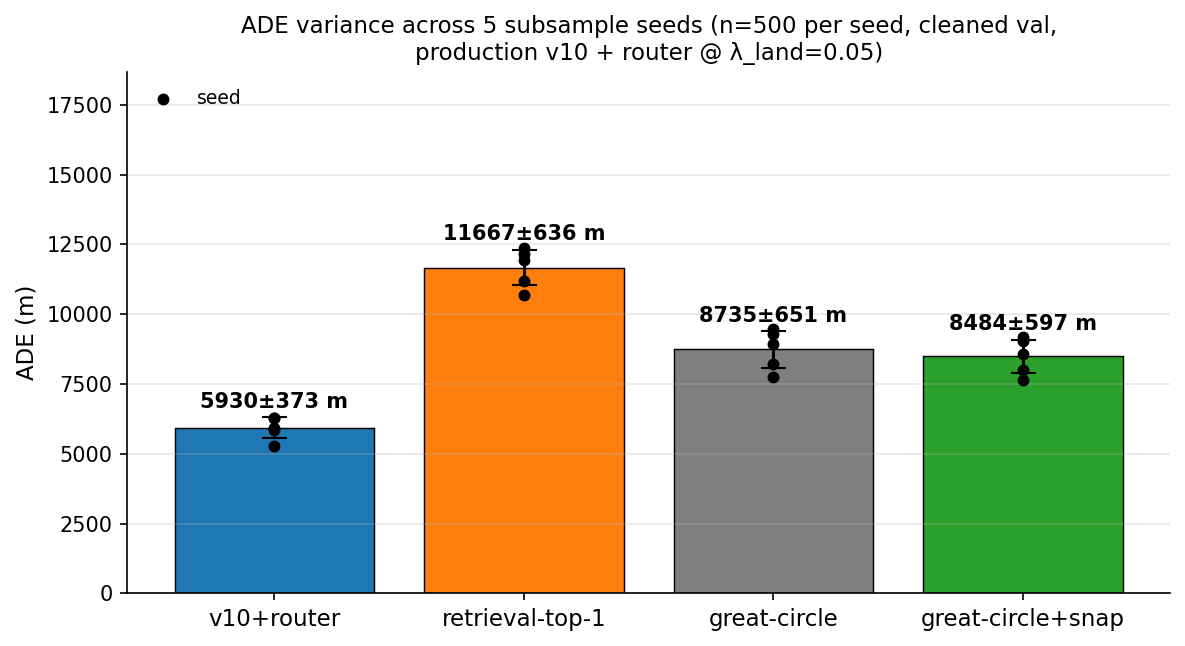
\includegraphics[width=0.78\linewidth]{figures/seed_variance.png}
\caption{Production \ade{} variance across five subsample seeds
         ($\{0,1,2,42,123\}$, $n=500$ each) on clean data.
         Black dots are individual seeds; error bars are $\pm 1\sigma$.
         The headline seed=42 figure (6282\,m) lies inside the
         v10\,+\,WaterRouter $\pm\sigma$ band (6052\,$\pm$\,225\,m),
         so the production claim is not seed-cherry-picked.
         Retrieval-top-1 degrades sharply on clean data because the clean
         corpus is 70\,\% smaller than the dirty one --- nearest-neighbour
         retrieval depends on corpus density.
         Full per-seed numbers are in Appendix~\ref{app:variance}.}
\label{fig:seed-variance-body}
\end{figure}

% =====================================================================
\section{Summary and Conclusion}
\label{sec:conclusion}

\subsection{What was achieved}

Starting from a next-step displacement predictor that could not beat a
constant-velocity baseline, this project arrived at:

\begin{itemize}
  \item A systematic study of \textbf{next-step displacement prediction}
        (v1) covering causal vs.\ bidirectional attention, displacement vs.\
        velocity targets, vessel-type embeddings, and lighthouse / nearest-vessel
        auxiliary features --- yielding the negative result that constant
        velocity is a near-optimal baseline on post-turn-segmented open-sea
        tracks, and the methodological lesson that motivated the move to
        full-sequence generation.
  \item An \textbf{architectural ladder for conditional route generation}
        (v2--v5) including a two-pass parallel formulation of scheduled
        sampling, bearing-feature conditioning, and a linear endpoint
        correction that drives FDE to zero without retraining.
  \item \textbf{Retrieval-augmented decoding} (v9, v10) ---
        per-timestep retrieval over a 163-token memory combined with a
        windowed causal mask and a differentiable land loss computed by
        bilinear interpolation on a 0.05$^{\circ}$ signed-distance raster.
  \item A production route generator (v10 + WaterRouter) achieving
        \ade{} = 6282\,m with 0\,\% land-crossing at the 10\,km threshold,
        running at $\sim$50\,ms per query on a CPU.
  \item Reusable infrastructure: a differentiable land SDF, a fine-resolution
        water-cell graph and A*/BFS router, and a retrieval substrate that
        can be reused by any future model (including v13).
  \item A full data pipeline from raw NOAA AIS downloads to evaluation-ready
        NPZ datasets, including E1 land filtering and KNN-cache construction.
  \item Detailed post-mortems for six failed or parked model variants
        (v6/v7/v8, v11, v12), surfacing reusable design principles
        for future generative-routing work.
\end{itemize}

\subsection{Open challenges}

Three structural problems remain unsolved:

\begin{enumerate}
\item \textbf{Multimodality.}  ADE measures distance to a single ground-truth route.
      A model that generates one high-quality mode of the route distribution will
      appear worse than one that generates the mean, even if the mode is more useful.
      Addressing this requires a coverage metric and a generative (non-deterministic)
      model --- motivating v13.
\item \textbf{Long-route degradation.}  No trained model has matched retrieval-top-1
      on routes $>$500\,km.  The mean-pool failure (v9) was fixed in v10, but v10's
      long-bucket \ade{} remains 1.4$\times$ worse than retrieval-top-1 on dirty data.
      A length router partially mitigates this without training.
\item \textbf{Hard water-validity at zero ADE cost.}
      All current approaches pay an ADE cost for enforcing the water constraint:
      $+5$\,\% for hard-projection on clean data, $\approx$0\,\% for snap-only
      on clean data (production).
      A model that structurally cannot generate land-crossing routes
      while maintaining ADE competitive with v9 remains an open problem.
\end{enumerate}

\subsection{The project's deepest lesson}

The single most repeated finding is:
\textbf{per-step training metrics do not predict autoregressive rollout quality.}
v2$\to$v5 demonstrated this on val\_delta; v12 demonstrated it again on CE accuracy.
Any proposed architecture should be validated by rollout evaluation at the smallest
reasonable scale before committing to a full training run.
This principle directly informs the v13 pre-flight checklist (Section~\ref{sec:future}).

% =====================================================================
\section{Outlook: Proposed v13 -- TrajDiff}
\label{sec:future}

\subsection{Motivation}

The v10 + WaterRouter production system is autoregressive: it generates one
waypoint at a time, conditioning on all previously generated waypoints.
This structure couples error propagation across all 128 steps (the source of
long-route degradation) and cannot natively sample multiple diverse routes
(limiting coverage of the multimodal distribution).

TrajDiff abandons autoregressive decoding in favour of
\emph{whole-sequence denoising diffusion}, reframing route generation as:
``start from a Gaussian noise trajectory and iteratively denoise it into a
plausible route, conditioning on (start, end, vessel-type, 5 retrieved routes).''
Diffusion models naturally support:
(1) multiple independent samples per query (diversity without retraining),
(2) inference-time guidance (land penalty applied at each DDIM step),
(3) the same conditioning bank as v10 (reusing verified retrieval infrastructure).

\subsection{Architecture overview}

A DiT~\cite{peebles2023dit} backbone with 6 bidirectional self-attention blocks
($d=256$, 8 heads, 1024-dim FFN, adaLN-Zero modulation by diffusion timestep).
The conditioning memory (same 163-token v10 bank) is provided via cross-attention.
SDF features (5$\times$5 coarse patch + 3$\times$3 fine patch at each of 128 noisy
positions) are computed per block and concatenated with the per-step input.
Classifier-free guidance with $p_\text{drop}=0.1$ and $w=1.5$.
Score-based land guidance adds $\eta_t \cdot \nabla_{x_t} \text{ReLU}(\text{sdf}-5)^2$
at each DDIM step, with $\eta_t$ annealed from 0 to 0.1.
At inference, 8 trajectories are sampled in parallel and the best-scoring is returned.

\begin{figure}[t]
\centering
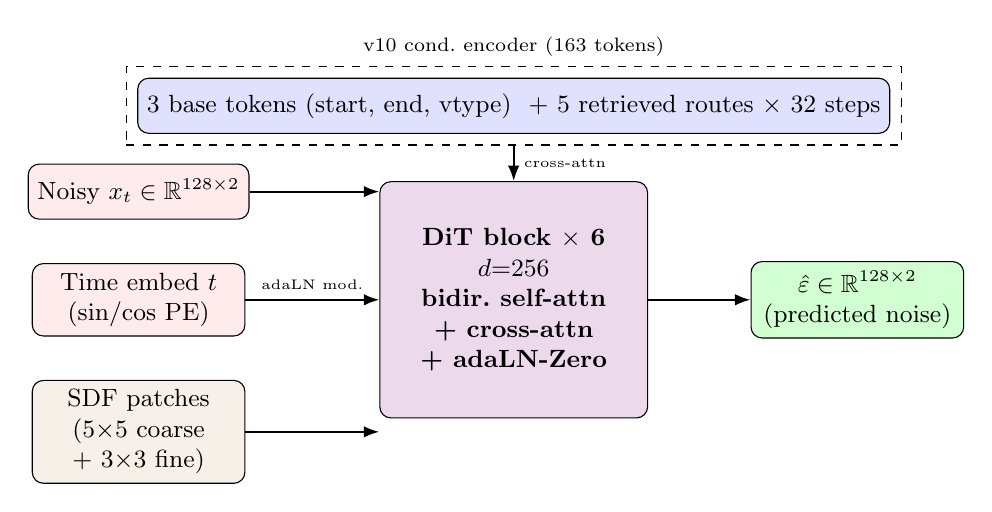
\begin{tikzpicture}[
    node distance=0.55cm and 1.2cm,
    box/.style={draw, rounded corners, minimum width=2.7cm, minimum height=0.7cm,
                align=center, font=\small},
    cond/.style={box, fill=blue!12, minimum width=3.6cm},
    noise/.style={box, fill=red!8},
    sdf/.style={box, fill=brown!12},
    dit/.style={box, fill=violet!15, minimum width=3.4cm, minimum height=3.0cm,
                align=center, font=\small\bfseries},
    outbox/.style={box, fill=green!18},
    arr/.style={-{Latex[scale=0.85]}, thick},
  ]
  % Noise input + time + SDF feats (LEFT column, stacked)
  \node[noise]                       (xt)  {Noisy $x_t \in \mathbb{R}^{128\times2}$};
  \node[noise, below=of xt]          (tt)  {Time embed $t$\\(sin/cos PE)};
  \node[sdf,   below=of tt]          (sf)  {SDF patches\\($5{\times}5$ coarse\\$+\ 3{\times}3$ fine)};
  % DiT block (to the right of xt/tt/sf)
  \node[dit, right=1.7cm of tt]      (dit) {DiT block $\times$ 6\\$d{=}256$\\bidir.\ self-attn\\+ cross-attn\\+ adaLN-Zero};
  % Conditioning encoder (ABOVE the DiT block; arrow comes down into it)
  \node[cond, above=0.6cm of dit]    (base) {3 base tokens (start, end, vtype)
                                               \ +\ 5 retrieved routes $\times$ 32 steps};
  \node[draw, dashed, fit=(base), inner sep=4pt,
        label=above:{\scriptsize v10 cond.\ encoder (163 tokens)}]
                                     (cbox) {};
  % Output (RIGHT of DiT)
  \node[outbox, right=1.3cm of dit]  (out) {$\hat\varepsilon \in \mathbb{R}^{128\times2}$\\(predicted noise)};

  % Arrows -- all terminate on named anchors.
  \draw[arr] (xt.east) -- (dit.west |- xt);
  \draw[arr] (tt.east) -- node[midway, above, font=\tiny] {adaLN mod.} (dit.west);
  \draw[arr] (sf.east) -- (dit.west |- sf);
  \draw[arr] (cbox.south) -- node[midway, right, font=\tiny] {cross-attn} (dit.north);
  \draw[arr] (dit.east) -- (out.west);
\end{tikzpicture}
\caption{v13 TrajDiff architecture (planned; not yet implemented).
         A bidirectional DiT denoises a 128-point noisy trajectory in normalised
         lon/lat space, conditioning on the same 163-token retrieval bank used by
         v10 (cross-attention) and on multi-scale SDF features sampled at the
         noisy positions (concatenated with the time embedding).
         At sample time, 8 trajectories are drawn in parallel, ranked by
         distance to the retrieval-top-1 neighbour minus a penalty for land
         crossings, and the best returned.
         The conditioning encoder (top) is reused verbatim from v10
         (Figure~\ref{fig:v10-arch}), so the v10 retrieval substrate transfers
         into the diffusion setting without re-training the encoder.}
\label{fig:v13-arch}
\end{figure}

\subsection{Length router (v13a)}

Independent of the trained model, a no-training length router dispatches on
great-circle distance:
\[
  \hat{\mathbf{x}} = \begin{cases}
    \text{retrieval-top-1} & \text{if } d_\text{GC} > 500\,km \\
    \text{v10 raw}         & \text{otherwise}
  \end{cases}
\]
Projected \ade{}: 5500--5800\,m on dirty data, based on the per-bucket
performance of v10 raw and retrieval-top-1 reported in Section~\ref{sec:results}.
This baseline must be evaluated before committing to v13 training: if the length
router already clears the target, the full diffusion model is unnecessary.

\subsection{Pre-flight checklist}

The engineering specification in \texttt{docs/v13\_proposal.md} lists five
pre-flight checks required before the 100-epoch training run:
\begin{enumerate}
  \item Re-evaluate v10 across seeds $\{0, 1, 7, 42, 100\}$ on clean data to
        measure $\sigma_\ade{}$ (required to determine statistical significance
        of any v13 improvement).
  \item Implement and evaluate the length router (v13a) without the trained model.
  \item Build \texttt{land\_sdf\_005deg.npz} and verify memory budget
        ($\approx$2.3\,GB at float16).
  \item Train a minimal unconditional DiT on $T=16$ (downsampled trajectories)
        for 20 epochs to confirm diffusion dynamics before scaling.
  \item Only then scale to $T=128$ with full conditioning.
\end{enumerate}

\textbf{v13 is specified but not yet implemented.}
All code described in this section (\texttt{src/model\_gen\_v13.py},
\texttt{src/diffusion.py}, training and eval scripts) remains to be written.

% =====================================================================
\bibliographystyle{plain}
\bibliography{references}

% =====================================================================
\appendix

\section{Reproducibility Notes}
\label{app:repro}

The production result (v10 + WaterRouter on clean data, ADE 6282\,m,
0\,\% land@10km) can be reproduced from the repository root as follows.

\textbf{Step 1: One-shot data builds (cached; skip if files exist):}
\begin{lstlisting}[language=bash]
python3 scripts/data/filter_trajgen_npz.py \
    --out_npz data/processed/trajgen_128_clean.npz \
    --land5_max_frac 0.02 --max_pen_km 10.0

python3 -c "from src.data_gen_retrieval import build_and_cache_knn; \
    build_and_cache_knn('data/processed/trajgen_128_clean.npz', \
                        'data/processed/trajgen_128_clean_knn_k5.npz', \
                        val_frac=0.15, seed=42, k=5, vtype_weight=0.5)"
\end{lstlisting}

\textbf{Step 2: Production evaluation (v10 ep52 checkpoint, no retraining):}
\begin{lstlisting}[language=bash]
python3 scripts/eval/eval_gen_v10_router.py \
    --data_npz data/processed/trajgen_128_clean.npz \
    --checkpoint runs/trajgen_v10/best.pt \
    --knn_cache data/processed/trajgen_128_clean_knn_k5.npz \
    --water_graph data/processed/water_graph_005deg.npz \
    --land_sdf data/processed/land_sdf_050deg.npz \
    --n_eval 500 --no_frechet
\end{lstlisting}

\textbf{Step 3: Regenerate report figures:}
\begin{lstlisting}[language=bash]
python3 scripts/eval/plot_comparison.py --out_dir figures/
python3 scripts/eval/plot_land_sdf.py \
    --land_sdf data/processed/land_sdf_050deg.npz \
    --out figures/land_sdf.png
cp figures/*.png report/figures/
cd report && latexmk -pdf report.tex
\end{lstlisting}

\textbf{Multi-seed variance.}  The single-seed limitation flagged in earlier
drafts has been resolved: \texttt{scripts/eval/multi\_seed\_variance.py} now
sweeps seeds $\{0, 1, 2, 42, 123\}$ on clean data and produces
\texttt{results/seed\_variance.csv}, \texttt{results/seed\_variance\_summary.txt},
and \texttt{figures/seed\_variance.png} (Appendix~\ref{app:variance}).

\textbf{Remaining limitations:}
\begin{itemize}
  \item Variance is over subsample selection ($n=500$ draws from the full val
        pool of $\sim$8.8\,k routes), not over training seeds.  Only one v10
        training was carried out.
  \item The displacement model (v1) baseline uses \texttt{results/baseline.json}
        saved per run; trajectory generation models do not produce this file
        (different evaluation protocol).
  \item The \texttt{12mo\_seq80.yaml} displacement config has no corresponding run
        (\texttt{runs/12mo\_seq80/} is empty) --- this run was never executed.
\end{itemize}

\section{Repository Structure}
\label{app:structure}

Key paths relative to the repository root:

\begin{description}
  \item[\texttt{src/}] Model and data modules.
        \texttt{model.py}/\texttt{data.py}/\texttt{metrics.py} (v1);
        \texttt{*\_gen.py} (v2); \texttt{*\_gen\_obs.py} (v6/v7);
        \texttt{*\_gen\_retrieval.py} (v9);
        \texttt{model\_gen\_v10.py}/\texttt{land\_mask.py}/\texttt{water\_router.py} (v10, production);
        \texttt{model\_gen\_v11.py}/\texttt{candidates.py} (v11, parked);
        \texttt{model\_gen\_v12.py}/\texttt{data\_gen\_v12.py} (v12, abandoned).
  \item[\texttt{scripts/train/}] One training script per model version.
  \item[\texttt{scripts/eval/}] Evaluation, visualisation, and plotting scripts.
  \item[\texttt{configs/}] YAML experiment configs grouped by approach
        (\texttt{displacement/}, \texttt{trajgen/}, \texttt{obstacle/}, \texttt{retrieval/}).
  \item[\texttt{runs/}] Training outputs (not tracked by git):
        \texttt{best.pt}, \texttt{metrics.csv}, \texttt{training\_curves.png} per run.
  \item[\texttt{data/processed/}] Processed datasets and cached artefacts (not tracked).
  \item[\texttt{docs/}] \texttt{narrative.md} (project narrative §1--§8);
        \texttt{decisions.md} (post-mortems); \texttt{v13\_proposal.md} (engineering spec);
        \texttt{references/} (three reference PDFs and notes).
  \item[\texttt{results/summary.csv}] One row per completed experiment with ADE/FDE
        and qualitative notes.
\end{description}

\section{Multi-seed variance of the production result}
\label{app:variance}

The headline production result reported in Section~\ref{sec:ranking}
(\ade{} = 6282\,m for v10\,+\,WaterRouter snap-only on
\texttt{trajgen\_128\_clean.npz}, $n{=}500$, seed\,$=42$) is supported by
four additional seed runs.  Each seed selects a different 500-route
subsample from the same val pool, so the figures probe how sensitive the
headline number is to which 500 routes happened to be drawn.

Concretely, \texttt{scripts/eval/multi\_seed\_variance.py} takes the union of
five 500-route subsamples (seeds $\{0, 1, 2, 42, 123\}$, totalling 2240
unique val routes out of 8783), runs v10 inference and the WaterRouter snap
once on the union, then slices to each seed and recomputes \ade{},
\fde{}, and the 10\,km land-crossing rate.
Table~\ref{tab:variance} reports the per-seed numbers;
Figure~\ref{fig:seed-variance-body} (in the main text) plots the production
ADE with $\pm 1\sigma$ error bars.

\begin{table}[ht]
\centering
\caption{Per-seed evaluation of the three core methods on clean data.
         v10\,+\,WaterRouter and retrieval-top-1 both reach exactly 0\,\%
         land-crossing (the corpus and the post-processor are
         water-structural).  Means are unweighted over the five seeds.}
\label{tab:variance}
\small
\begin{tabular}{lrrr|rrr|rrr}
\toprule
seed & \multicolumn{3}{c}{v10\,+\,WaterRouter} & \multicolumn{3}{c}{Retrieval-top-1} & \multicolumn{3}{c}{Great-circle} \\
     & \ade{} & \fde{} & cross\% & \ade{} & \fde{} & cross\% & \ade{} & \fde{} & cross\% \\
\midrule
  0  &  6035 &  575 & 0.0 & 12170 & 12428 & 0.0 &  9459 & 0.1 &  9.4 \\
  1  &  6106 &  594 & 0.0 & 10680 & 11408 & 0.0 &  8202 & 0.1 &  8.0 \\
  2  &  5633 &  567 & 0.0 & 11190 & 11234 & 0.0 &  7763 & 0.1 &  8.0 \\
 42  &  6282 &  561 & 0.0 & 12374 & 12283 & 0.0 &  9304 & 0.1 &  9.0 \\
123  &  6201 &  606 & 0.0 & 11922 & 11809 & 0.0 &  8949 & 0.1 &  9.6 \\
\midrule
mean $\pm$ std & $6052 \pm 225$ & $581 \pm 17$ & 0.0 & $11667 \pm 636$ & $11832 \pm 469$ & 0.0 & $8735 \pm 651$ & 0.1 & $8.8 \pm 0.7$ \\
\bottomrule
\end{tabular}
\end{table}

\textbf{What this rules out.}
Any future improvement of less than $\sim$225\,m in \ade{} is not
statistically distinguishable from this seed noise floor; report claims
below that bar should not be reported as headline improvements.

\textbf{What this still does not measure.}
This is variance over \emph{which 500 routes were drawn}, not over training
seeds (only one training seed was used for v10).
Measuring training-seed variance would require multiple full v10 trainings,
which exceeds the project's compute budget; it is recorded as future work
in the v13 pre-flight checklist (Section~\ref{sec:future}).

\end{document}
